\documentclass[twoside]{book}

% Packages required by doxygen
\usepackage{fixltx2e}
\usepackage{calc}
\usepackage{doxygen}
\usepackage[export]{adjustbox} % also loads graphicx
\usepackage{graphicx}
\usepackage[utf8]{inputenc}
\usepackage{makeidx}
\usepackage{multicol}
\usepackage{multirow}
\PassOptionsToPackage{warn}{textcomp}
\usepackage{textcomp}
\usepackage[nointegrals]{wasysym}
\usepackage[table]{xcolor}

% NLS support packages
\usepackage[french]{babel}

% Font selection
\usepackage[T1]{fontenc}
\usepackage[scaled=.90]{helvet}
\usepackage{courier}
\usepackage{amssymb}
\usepackage{sectsty}
\renewcommand{\familydefault}{\sfdefault}
\allsectionsfont{%
  \fontseries{bc}\selectfont%
  \color{darkgray}%
}
\renewcommand{\DoxyLabelFont}{%
  \fontseries{bc}\selectfont%
  \color{darkgray}%
}
\newcommand{\+}{\discretionary{\mbox{\scriptsize$\hookleftarrow$}}{}{}}

% Page & text layout
\usepackage{geometry}
\geometry{%
  a4paper,%
  top=2.5cm,%
  bottom=2.5cm,%
  left=2.5cm,%
  right=2.5cm%
}
\tolerance=750
\hfuzz=15pt
\hbadness=750
\setlength{\emergencystretch}{15pt}
\setlength{\parindent}{0cm}
\setlength{\parskip}{3ex plus 2ex minus 2ex}
\makeatletter
\renewcommand{\paragraph}{%
  \@startsection{paragraph}{4}{0ex}{-1.0ex}{1.0ex}{%
    \normalfont\normalsize\bfseries\SS@parafont%
  }%
}
\renewcommand{\subparagraph}{%
  \@startsection{subparagraph}{5}{0ex}{-1.0ex}{1.0ex}{%
    \normalfont\normalsize\bfseries\SS@subparafont%
  }%
}
\makeatother

% Headers & footers
\usepackage{fancyhdr}
\pagestyle{fancyplain}
\fancyhead[LE]{\fancyplain{}{\bfseries\thepage}}
\fancyhead[CE]{\fancyplain{}{}}
\fancyhead[RE]{\fancyplain{}{\bfseries\leftmark}}
\fancyhead[LO]{\fancyplain{}{\bfseries\rightmark}}
\fancyhead[CO]{\fancyplain{}{}}
\fancyhead[RO]{\fancyplain{}{\bfseries\thepage}}
\fancyfoot[LE]{\fancyplain{}{}}
\fancyfoot[CE]{\fancyplain{}{}}
\fancyfoot[RE]{\fancyplain{}{\bfseries\scriptsize Généré par Doxygen }}
\fancyfoot[LO]{\fancyplain{}{\bfseries\scriptsize Généré par Doxygen }}
\fancyfoot[CO]{\fancyplain{}{}}
\fancyfoot[RO]{\fancyplain{}{}}
\renewcommand{\footrulewidth}{0.4pt}
\renewcommand{\chaptermark}[1]{%
  \markboth{#1}{}%
}
\renewcommand{\sectionmark}[1]{%
  \markright{\thesection\ #1}%
}

% Indices & bibliography
\usepackage{natbib}
\usepackage[titles]{tocloft}
\setcounter{tocdepth}{3}
\setcounter{secnumdepth}{5}
\makeindex

% Hyperlinks (required, but should be loaded last)
\usepackage{ifpdf}
\ifpdf
  \usepackage[pdftex,pagebackref=true]{hyperref}
\else
  \usepackage[ps2pdf,pagebackref=true]{hyperref}
\fi
\hypersetup{%
  colorlinks=true,%
  linkcolor=blue,%
  citecolor=blue,%
  unicode%
}

% Custom commands
\newcommand{\clearemptydoublepage}{%
  \newpage{\pagestyle{empty}\cleardoublepage}%
}

\usepackage{caption}
\captionsetup{labelsep=space,justification=centering,font={bf},singlelinecheck=off,skip=4pt,position=top}

%===== C O N T E N T S =====

\begin{document}

% Titlepage & ToC
\hypersetup{pageanchor=false,
             bookmarksnumbered=true,
             pdfencoding=unicode
            }
\pagenumbering{roman}
\begin{titlepage}
\vspace*{7cm}
\begin{center}%
{\Large Robot distributeur de Café }\\
\vspace*{1cm}
{\large Généré par Doxygen 1.8.11}\\
\end{center}
\end{titlepage}
\clearemptydoublepage
\tableofcontents
\clearemptydoublepage
\pagenumbering{arabic}
\hypersetup{pageanchor=true}

%--- Begin generated contents ---
\chapter{Index des classes}
\section{Class List}
Here are the classes, structs, unions and interfaces with brief descriptions\+:\begin{DoxyCompactList}
\item\contentsline{section}{\hyperlink{classdecision}{decision} }{\pageref{classdecision}}{}
\item\contentsline{section}{\hyperlink{classmoving__persons__detector}{moving\+\_\+persons\+\_\+detector} }{\pageref{classmoving__persons__detector}}{}
\item\contentsline{section}{\hyperlink{classobstacle__detection}{obstacle\+\_\+detection} }{\pageref{classobstacle__detection}}{}
\item\contentsline{section}{\hyperlink{classrobot__moving__lectures}{robot\+\_\+moving\+\_\+lectures} }{\pageref{classrobot__moving__lectures}}{}
\item\contentsline{section}{\hyperlink{classrotation__action}{rotation\+\_\+action} }{\pageref{classrotation__action}}{}
\item\contentsline{section}{\hyperlink{classtranslation__action}{translation\+\_\+action} }{\pageref{classtranslation__action}}{}
\end{DoxyCompactList}

\chapter{Index des fichiers}
\section{File List}
Here is a list of all documented files with brief descriptions\+:\begin{DoxyCompactList}
\item\contentsline{section}{/home/maxence/robair/src/follow\+\_\+me/src/\hyperlink{decision__node_8cpp}{decision\+\_\+node.\+cpp} \\*Noeud de décision }{\pageref{decision__node_8cpp}}{}
\end{DoxyCompactList}

\chapter{Documentation des classes}
\hypertarget{classdecision}{}\section{decision Class Reference}
\label{classdecision}\index{decision@{decision}}
\subsection*{Public Member Functions}
\begin{DoxyCompactItemize}
\item 
\hyperlink{classdecision_a00772c969f42d590e57f3eb37bafe6a6}{decision} ()
\item 
void \hyperlink{classdecision_a5fbd0cdaffc906d31560227560136b59}{update} ()\hypertarget{classdecision_a5fbd0cdaffc906d31560227560136b59}{}\label{classdecision_a5fbd0cdaffc906d31560227560136b59}

\begin{DoxyCompactList}\small\item\em Met à jour le noeud. \end{DoxyCompactList}\item 
void {\bfseries send\+\_\+finish\+\_\+move} (bool b)\hypertarget{classdecision_adabd8116029927f426558cbc87acba0e}{}\label{classdecision_adabd8116029927f426558cbc87acba0e}

\item 
void \hyperlink{classdecision_afddf261c387d28dde5e6881343518ca7}{goal\+\_\+to\+\_\+reach\+Callback} (const geometry\+\_\+msgs\+::\+Point\+::\+Const\+Ptr \&g)
\begin{DoxyCompactList}\small\item\em Callback pour l\textquotesingle{}inscription au topic goal\+\_\+to\+\_\+reach. \end{DoxyCompactList}\item 
void \hyperlink{classdecision_ad6c2257e2304ad3a078d2b64cf425caa}{rotation\+\_\+done\+Callback} (const std\+\_\+msgs\+::\+Float32\+::\+Const\+Ptr \&a)
\begin{DoxyCompactList}\small\item\em Callback pour l\textquotesingle{}inscription au rotation\+\_\+done. \end{DoxyCompactList}\item 
void {\bfseries token\+\_\+\+Callback} (const std\+\_\+msgs\+::\+Bool\+::\+Const\+Ptr \&a)\hypertarget{classdecision_a7e0da40a27e1c320329a5b81f6044c57}{}\label{classdecision_a7e0da40a27e1c320329a5b81f6044c57}

\item 
void \hyperlink{classdecision_ab874f222aac437a05fe8bc8c5d8963b4}{translation\+\_\+done\+Callback} (const std\+\_\+msgs\+::\+Float32\+::\+Const\+Ptr \&r)
\begin{DoxyCompactList}\small\item\em Callback pour l\textquotesingle{}inscription au translation\+\_\+done. \end{DoxyCompactList}\item 
float \hyperlink{classdecision_a1b6988efc70e0a25ddb7be0f372d2ad2}{distance\+Points} (geometry\+\_\+msgs\+::\+Point pa, geometry\+\_\+msgs\+::\+Point pb)
\begin{DoxyCompactList}\small\item\em Revoie la distance entre deux points. \end{DoxyCompactList}\end{DoxyCompactItemize}


\subsection{Constructor \& Destructor Documentation}
\index{decision@{decision}!decision@{decision}}
\index{decision@{decision}!decision@{decision}}
\subsubsection[{\texorpdfstring{decision()}{decision()}}]{\setlength{\rightskip}{0pt plus 5cm}decision\+::decision (
\begin{DoxyParamCaption}
{}
\end{DoxyParamCaption}
)\hspace{0.3cm}{\ttfamily [inline]}}\hypertarget{classdecision_a00772c969f42d590e57f3eb37bafe6a6}{}\label{classdecision_a00772c969f42d590e57f3eb37bafe6a6}
Constructeur de la classe Decision 

\subsection{Member Function Documentation}
\index{decision@{decision}!distance\+Points@{distance\+Points}}
\index{distance\+Points@{distance\+Points}!decision@{decision}}
\subsubsection[{\texorpdfstring{distance\+Points(geometry\+\_\+msgs\+::\+Point pa, geometry\+\_\+msgs\+::\+Point pb)}{distancePoints(geometry_msgs::Point pa, geometry_msgs::Point pb)}}]{\setlength{\rightskip}{0pt plus 5cm}decision\+::distance\+Points (
\begin{DoxyParamCaption}
\item[{geometry\+\_\+msgs\+::\+Point}]{pa, }
\item[{geometry\+\_\+msgs\+::\+Point}]{pb}
\end{DoxyParamCaption}
)\hspace{0.3cm}{\ttfamily [inline]}}\hypertarget{classdecision_a1b6988efc70e0a25ddb7be0f372d2ad2}{}\label{classdecision_a1b6988efc70e0a25ddb7be0f372d2ad2}


Revoie la distance entre deux points. 


\begin{DoxyParams}{Parameters}
{\em pa} & le premier point \\
\hline
{\em pb} & le second point \\
\hline
\end{DoxyParams}
\begin{DoxyReturn}{Returns}
la distance entre le point pa et le point pb 
\end{DoxyReturn}
\index{decision@{decision}!goal\+\_\+to\+\_\+reach\+Callback@{goal\+\_\+to\+\_\+reach\+Callback}}
\index{goal\+\_\+to\+\_\+reach\+Callback@{goal\+\_\+to\+\_\+reach\+Callback}!decision@{decision}}
\subsubsection[{\texorpdfstring{goal\+\_\+to\+\_\+reach\+Callback(const geometry\+\_\+msgs\+::\+Point\+::\+Const\+Ptr \&g)}{goal_to_reachCallback(const geometry_msgs::Point::ConstPtr &g)}}]{\setlength{\rightskip}{0pt plus 5cm}decision\+::goal\+\_\+to\+\_\+reach\+Callback (
\begin{DoxyParamCaption}
\item[{const geometry\+\_\+msgs\+::\+Point\+::\+Const\+Ptr \&}]{g}
\end{DoxyParamCaption}
)\hspace{0.3cm}{\ttfamily [inline]}}\hypertarget{classdecision_afddf261c387d28dde5e6881343518ca7}{}\label{classdecision_afddf261c387d28dde5e6881343518ca7}


Callback pour l\textquotesingle{}inscription au topic goal\+\_\+to\+\_\+reach. 


\begin{DoxyParams}{Parameters}
{\em g} & le point reçu \\
\hline
\end{DoxyParams}
\index{decision@{decision}!rotation\+\_\+done\+Callback@{rotation\+\_\+done\+Callback}}
\index{rotation\+\_\+done\+Callback@{rotation\+\_\+done\+Callback}!decision@{decision}}
\subsubsection[{\texorpdfstring{rotation\+\_\+done\+Callback(const std\+\_\+msgs\+::\+Float32\+::\+Const\+Ptr \&a)}{rotation_doneCallback(const std_msgs::Float32::ConstPtr &a)}}]{\setlength{\rightskip}{0pt plus 5cm}decision\+::rotation\+\_\+done\+Callback (
\begin{DoxyParamCaption}
\item[{const std\+\_\+msgs\+::\+Float32\+::\+Const\+Ptr \&}]{a}
\end{DoxyParamCaption}
)\hspace{0.3cm}{\ttfamily [inline]}}\hypertarget{classdecision_ad6c2257e2304ad3a078d2b64cf425caa}{}\label{classdecision_ad6c2257e2304ad3a078d2b64cf425caa}


Callback pour l\textquotesingle{}inscription au rotation\+\_\+done. 


\begin{DoxyParams}{Parameters}
{\em a} & l\textquotesingle{}angle parcouru \\
\hline
\end{DoxyParams}
\index{decision@{decision}!translation\+\_\+done\+Callback@{translation\+\_\+done\+Callback}}
\index{translation\+\_\+done\+Callback@{translation\+\_\+done\+Callback}!decision@{decision}}
\subsubsection[{\texorpdfstring{translation\+\_\+done\+Callback(const std\+\_\+msgs\+::\+Float32\+::\+Const\+Ptr \&r)}{translation_doneCallback(const std_msgs::Float32::ConstPtr &r)}}]{\setlength{\rightskip}{0pt plus 5cm}decision\+::translation\+\_\+done\+Callback (
\begin{DoxyParamCaption}
\item[{const std\+\_\+msgs\+::\+Float32\+::\+Const\+Ptr \&}]{r}
\end{DoxyParamCaption}
)\hspace{0.3cm}{\ttfamily [inline]}}\hypertarget{classdecision_ab874f222aac437a05fe8bc8c5d8963b4}{}\label{classdecision_ab874f222aac437a05fe8bc8c5d8963b4}


Callback pour l\textquotesingle{}inscription au translation\+\_\+done. 


\begin{DoxyParams}{Parameters}
{\em r} & distance effectuée \\
\hline
\end{DoxyParams}


The documentation for this class was generated from the following file\+:\begin{DoxyCompactItemize}
\item 
/home/maxence/robair/src/follow\+\_\+me/src/\hyperlink{decision__node_8cpp}{decision\+\_\+node.\+cpp}\end{DoxyCompactItemize}

\hypertarget{classmoving__persons__detector}{}\section{Référence de la classe moving\+\_\+persons\+\_\+detector}
\label{classmoving__persons__detector}\index{moving\+\_\+persons\+\_\+detector@{moving\+\_\+persons\+\_\+detector}}


Détecte les personnes et les groupes.  


\subsection*{Fonctions membres publiques}
\begin{DoxyCompactItemize}
\item 
\hyperlink{classmoving__persons__detector_ab7d7bf4e0edf8a64a8a43e0a8dad3083}{moving\+\_\+persons\+\_\+detector} ()
\item 
void \hyperlink{classmoving__persons__detector_a7f3a34bf99f2070b44c3a2424a4a4559}{finish\+\_\+move\+\_\+\+Callback} (const std\+\_\+msgs\+::\+Bool\+::\+Const\+Ptr \&a)
\begin{DoxyCompactList}\small\item\em réception des messages du topic finish\+\_\+move \end{DoxyCompactList}\item 
void \hyperlink{classmoving__persons__detector_a83ca0ba4254abe369da899d54984502d}{update} ()
\begin{DoxyCompactList}\small\item\em Met à jour le noeud. \end{DoxyCompactList}\item 
void \hyperlink{classmoving__persons__detector_a8b1c0d12b9eca4cb94b195fbf5847726}{send\+\_\+goal\+\_\+to\+\_\+reach} ()
\begin{DoxyCompactList}\small\item\em envoie du but \end{DoxyCompactList}\item 
void \hyperlink{classmoving__persons__detector_a833595f068de84045e6d67ab68c474dd}{store\+\_\+background} ()
\begin{DoxyCompactList}\small\item\em Enregistre les points. \end{DoxyCompactList}\item 
void \hyperlink{classmoving__persons__detector_a5c0563104a7d043297d9db0a0fd1ad3f}{detect\+\_\+motion} ()
\begin{DoxyCompactList}\small\item\em detecte la mouvement des points \end{DoxyCompactList}\item 
void \hyperlink{classmoving__persons__detector_a985ef636f8e95332f1559681aff3414f}{perform\+\_\+clustering} ()
\begin{DoxyCompactList}\small\item\em Effectue le clustering des points. \end{DoxyCompactList}\item 
void \hyperlink{classmoving__persons__detector_ab84737ca7963b67f6aa8a9b9bf4322b0}{detect\+\_\+moving\+\_\+legs} ()
\begin{DoxyCompactList}\small\item\em Effectue la détection des jambes. \end{DoxyCompactList}\item 
void \hyperlink{classmoving__persons__detector_af1519f7b134ebe1742d4837b675f0810}{detect\+\_\+moving\+\_\+persons} ()
\begin{DoxyCompactList}\small\item\em Détect les personnes. \end{DoxyCompactList}\item 
geometry\+\_\+msgs\+::\+Point \hyperlink{classmoving__persons__detector_a56e54848546290d3dd0c06956763ee30}{closest\+\_\+group} ()
\begin{DoxyCompactList}\small\item\em renvoie le groupe le plus proche du robot \end{DoxyCompactList}\item 
void \hyperlink{classmoving__persons__detector_af5443988d657ef8a8491a31e5e8ec9fa}{scan\+Callback} (const sensor\+\_\+msgs\+::\+Laser\+Scan\+::\+Const\+Ptr \&scan)
\begin{DoxyCompactList}\small\item\em callback du scan du laser \end{DoxyCompactList}\item 
void \hyperlink{classmoving__persons__detector_adc5abaf5a29ad580e32491549e4cf784}{robot\+\_\+moving\+Callback} (const std\+\_\+msgs\+::\+Bool\+::\+Const\+Ptr \&state)
\begin{DoxyCompactList}\small\item\em callback de l\textquotesingle{}état du robot \end{DoxyCompactList}\item 
float \hyperlink{classmoving__persons__detector_a2724a72050ae34ba6d1a2804941d9758}{distance\+Points} (geometry\+\_\+msgs\+::\+Point pa, geometry\+\_\+msgs\+::\+Point pb)
\begin{DoxyCompactList}\small\item\em Revoie la distance entre deux points. \end{DoxyCompactList}\item 
void \hyperlink{classmoving__persons__detector_ab8a95eb655a08e7507bae53976739233}{populate\+Marker\+Reference} ()
\begin{DoxyCompactList}\small\item\em affichage des points \end{DoxyCompactList}\item 
void \hyperlink{classmoving__persons__detector_ac3ea794336284aefb88e9b78a3ce8f8f}{populate\+Marker\+Topic} ()
\begin{DoxyCompactList}\small\item\em affichage des points \end{DoxyCompactList}\item 
void \hyperlink{classmoving__persons__detector_aa198d0acd452104d0292c613af3ca520}{send\+\_\+token} (bool b)
\begin{DoxyCompactList}\small\item\em Envoie du token. \end{DoxyCompactList}\item 
void \hyperlink{classmoving__persons__detector_a73acba9d4ee78f4cfb1bf0659334cd49}{print\+\_\+sorce} ()
\begin{DoxyCompactList}\small\item\em affichage des scores \end{DoxyCompactList}\item 
void \hyperlink{classmoving__persons__detector_aa2f36db42b79877062d4d9326995eb4d}{reset\+\_\+score} ()
\begin{DoxyCompactList}\small\item\em Suppression des scores. \end{DoxyCompactList}\item 
void \hyperlink{classmoving__persons__detector_a963302ef27df7f685e48ab4d0c5cb674}{detect\+\_\+group} ()
\begin{DoxyCompactList}\small\item\em Recherche les différents groupes. \end{DoxyCompactList}\end{DoxyCompactItemize}
\subsection*{Attributs privés}
\begin{DoxyCompactItemize}
\item 
ros\+::\+Node\+Handle \hyperlink{classmoving__persons__detector_ac7ce090922b1fbb39792fe80249c2ac7}{n}
\item 
ros\+::\+Subscriber \hyperlink{classmoving__persons__detector_a4927f845c4631be26ced13aa0f306161}{sub\+\_\+scan}
\item 
ros\+::\+Subscriber \hyperlink{classmoving__persons__detector_a2ebd9075ece54b52335ba5aa7c7e073e}{sub\+\_\+robot\+\_\+moving}
\item 
ros\+::\+Subscriber \hyperlink{classmoving__persons__detector_a212ab693f8f575f3770d76efd51bb215}{sub\+\_\+finish\+\_\+move}
\item 
ros\+::\+Publisher \hyperlink{classmoving__persons__detector_a76a32d740a76752eb8d806ed50f1dbdd}{pub\+\_\+moving\+\_\+persons\+\_\+detector}
\item 
ros\+::\+Publisher \hyperlink{classmoving__persons__detector_adb07f5fa4d75d6c8f2e037a9b9e38e7a}{pub\+\_\+moving\+\_\+persons\+\_\+detector\+\_\+marker}
\item 
int \hyperlink{classmoving__persons__detector_ad6c97c267707ec5b67e3295899ccb40d}{nb\+\_\+beams}
\item 
float \hyperlink{classmoving__persons__detector_a92cf37109057a74bd655a7d4366c29e4}{range\+\_\+min}
\item 
float \hyperlink{classmoving__persons__detector_a93be1d4fd3177968890c7e8917f047ab}{range\+\_\+max}
\item 
float \hyperlink{classmoving__persons__detector_a57cb7dfbf0b886b6cfb87c0c9f9e4cf1}{angle\+\_\+min}
\item 
float \hyperlink{classmoving__persons__detector_acc6274815996d0b9e2882df73d951a17}{angle\+\_\+max}
\item 
float \hyperlink{classmoving__persons__detector_a87b53ed0ee82616d481cb0b68351f971}{angle\+\_\+inc}
\item 
float \hyperlink{classmoving__persons__detector_a07152a36a51361a3f7b7ebdf9cf809c1}{range} \mbox{[}1000\mbox{]}
\item 
geometry\+\_\+msgs\+::\+Point \hyperlink{classmoving__persons__detector_a8e17523454477a9e7ed1e87c9f42816b}{current\+\_\+scan} \mbox{[}1000\mbox{]}
\item 
bool \hyperlink{classmoving__persons__detector_a49ade373e545c987b519a7c2e686820c}{new\+\_\+goal}
\item 
float \hyperlink{classmoving__persons__detector_ab6c082d9a769d1065f400e449320c3ad}{background} \mbox{[}1000\mbox{]}
\item 
bool \hyperlink{classmoving__persons__detector_a32f205edd674741153028305da0103a2}{dynamic} \mbox{[}1000\mbox{]}
\item 
int \hyperlink{classmoving__persons__detector_a62bb0f7e285afa97978df71473259d58}{nb\+\_\+cluster}
\item 
int \hyperlink{classmoving__persons__detector_a8453207bfdcffd1e45ab9dcc73210e60}{cluster} \mbox{[}1000\mbox{]}
\item 
float \hyperlink{classmoving__persons__detector_ace70d87779974b46c12273865b36ccf1}{cluster\+\_\+size} \mbox{[}1000\mbox{]}
\item 
geometry\+\_\+msgs\+::\+Point \hyperlink{classmoving__persons__detector_a4a961028d83e2d74b5af1e53593be67c}{cluster\+\_\+middle} \mbox{[}1000\mbox{]}
\item 
int \hyperlink{classmoving__persons__detector_a729d1bcf6929766ce3a6e6f5fe0a56d1}{cluster\+\_\+dynamic} \mbox{[}1000\mbox{]}
\item 
int \hyperlink{classmoving__persons__detector_aa8bb9b30e452cb90530b96328f07d54a}{cluster\+\_\+start} \mbox{[}1000\mbox{]}
\item 
int \hyperlink{classmoving__persons__detector_a0d32b0ae38b8f9b26c007faabafe7450}{cluster\+\_\+end} \mbox{[}1000\mbox{]}
\item 
int \hyperlink{classmoving__persons__detector_aee7e42a55781f7c7297c7355296c6666}{nb\+\_\+moving\+\_\+legs\+\_\+detected}
\item 
geometry\+\_\+msgs\+::\+Point \hyperlink{classmoving__persons__detector_a412141d71e00568c403f083c9c7b5410}{moving\+\_\+leg\+\_\+detected} \mbox{[}1000\mbox{]}
\item 
int \hyperlink{classmoving__persons__detector_a7f2bae601889ce3c935ae218814e6be9}{nb\+\_\+moving\+\_\+persons\+\_\+detected}
\item 
geometry\+\_\+msgs\+::\+Point \hyperlink{classmoving__persons__detector_a20d0b31be1b975603b3967e8de6da662}{moving\+\_\+persons\+\_\+detected} \mbox{[}1000\mbox{]}
\item 
geometry\+\_\+msgs\+::\+Point \hyperlink{classmoving__persons__detector_af718cc27ac29e0ca034fbafe542cf23c}{goal\+\_\+to\+\_\+reach}
\item 
int \hyperlink{classmoving__persons__detector_a207858cf1fc0675c38eb41a5d8edf245}{nb\+\_\+pts}
\item 
geometry\+\_\+msgs\+::\+Point \hyperlink{classmoving__persons__detector_a7a74890a878182e5e70a7a72feb6b648}{display} \mbox{[}2000\mbox{]}
\item 
std\+\_\+msgs\+::\+Color\+R\+G\+BA \hyperlink{classmoving__persons__detector_af658a75f3cf4bd684fb2a282ce52af04}{colors} \mbox{[}2000\mbox{]}
\item 
bool \hyperlink{classmoving__persons__detector_a782b66e8437a7e2d8501d0eefe4eedc4}{previous\+\_\+robot\+\_\+moving}
\item 
bool \hyperlink{classmoving__persons__detector_ac3e2309e03a591892b8b13ba51df6831}{current\+\_\+robot\+\_\+moving}
\item 
ros\+::\+Publisher \hyperlink{classmoving__persons__detector_a8e87dbae89154f33ce2a2275c1599b10}{pub\+\_\+goal\+\_\+to\+\_\+reach}
\item 
bool \hyperlink{classmoving__persons__detector_a379e4d7d62fc6b2a163464b728177463}{new\+\_\+laser}
\item 
bool \hyperlink{classmoving__persons__detector_a4eace803293c56e7ee5b33093ea3cdea}{new\+\_\+robot}
\item 
ros\+::\+Publisher \hyperlink{classmoving__persons__detector_af6a77470dc3e40277e9e8e08d4afd7cf}{pub\+\_\+token}
\item 
int \hyperlink{classmoving__persons__detector_a798768403d1a8a3964ca22723fbd3918}{nb\+\_\+iter}
\item 
int \hyperlink{classmoving__persons__detector_ab92fa10f71867379e997220065b5ce38}{score} \mbox{[}1000\mbox{]}
\item 
int \hyperlink{classmoving__persons__detector_a7f33b7e0a227a032dc845a74cc805837}{nb\+\_\+group\+\_\+detected}
\item 
geometry\+\_\+msgs\+::\+Point \hyperlink{classmoving__persons__detector_a40e04cd6cda49ccc016b5881d048c46a}{group\+\_\+detected} \mbox{[}1000\mbox{]}
\item 
bool \hyperlink{classmoving__persons__detector_ab9eaeb335101abe8964220a7f41fdcab}{finish\+\_\+move}
\end{DoxyCompactItemize}


\subsection{Description détaillée}
Détecte les personnes et les groupes. 

\subsection{Documentation des constructeurs et destructeur}
\index{moving\+\_\+persons\+\_\+detector@{moving\+\_\+persons\+\_\+detector}!moving\+\_\+persons\+\_\+detector@{moving\+\_\+persons\+\_\+detector}}
\index{moving\+\_\+persons\+\_\+detector@{moving\+\_\+persons\+\_\+detector}!moving\+\_\+persons\+\_\+detector@{moving\+\_\+persons\+\_\+detector}}
\subsubsection[{\texorpdfstring{moving\+\_\+persons\+\_\+detector()}{moving_persons_detector()}}]{\setlength{\rightskip}{0pt plus 5cm}moving\+\_\+persons\+\_\+detector\+::moving\+\_\+persons\+\_\+detector (
\begin{DoxyParamCaption}
{}
\end{DoxyParamCaption}
)\hspace{0.3cm}{\ttfamily [inline]}}\hypertarget{classmoving__persons__detector_ab7d7bf4e0edf8a64a8a43e0a8dad3083}{}\label{classmoving__persons__detector_ab7d7bf4e0edf8a64a8a43e0a8dad3083}
Constructeur de la classe moving\+\_\+person\+\_\+detector 

\subsection{Documentation des fonctions membres}
\index{moving\+\_\+persons\+\_\+detector@{moving\+\_\+persons\+\_\+detector}!closest\+\_\+group@{closest\+\_\+group}}
\index{closest\+\_\+group@{closest\+\_\+group}!moving\+\_\+persons\+\_\+detector@{moving\+\_\+persons\+\_\+detector}}
\subsubsection[{\texorpdfstring{closest\+\_\+group()}{closest_group()}}]{\setlength{\rightskip}{0pt plus 5cm}geometry\+\_\+msgs\+::\+Point moving\+\_\+persons\+\_\+detector\+::closest\+\_\+group (
\begin{DoxyParamCaption}
{}
\end{DoxyParamCaption}
)\hspace{0.3cm}{\ttfamily [inline]}}\hypertarget{classmoving__persons__detector_a56e54848546290d3dd0c06956763ee30}{}\label{classmoving__persons__detector_a56e54848546290d3dd0c06956763ee30}


renvoie le groupe le plus proche du robot 

\begin{DoxyReturn}{Renvoie}
le groupe le plus proche 
\end{DoxyReturn}
\index{moving\+\_\+persons\+\_\+detector@{moving\+\_\+persons\+\_\+detector}!detect\+\_\+group@{detect\+\_\+group}}
\index{detect\+\_\+group@{detect\+\_\+group}!moving\+\_\+persons\+\_\+detector@{moving\+\_\+persons\+\_\+detector}}
\subsubsection[{\texorpdfstring{detect\+\_\+group()}{detect_group()}}]{\setlength{\rightskip}{0pt plus 5cm}void moving\+\_\+persons\+\_\+detector\+::detect\+\_\+group (
\begin{DoxyParamCaption}
{}
\end{DoxyParamCaption}
)\hspace{0.3cm}{\ttfamily [inline]}}\hypertarget{classmoving__persons__detector_a963302ef27df7f685e48ab4d0c5cb674}{}\label{classmoving__persons__detector_a963302ef27df7f685e48ab4d0c5cb674}


Recherche les différents groupes. 

\index{moving\+\_\+persons\+\_\+detector@{moving\+\_\+persons\+\_\+detector}!detect\+\_\+motion@{detect\+\_\+motion}}
\index{detect\+\_\+motion@{detect\+\_\+motion}!moving\+\_\+persons\+\_\+detector@{moving\+\_\+persons\+\_\+detector}}
\subsubsection[{\texorpdfstring{detect\+\_\+motion()}{detect_motion()}}]{\setlength{\rightskip}{0pt plus 5cm}moving\+\_\+persons\+\_\+detector\+::detect\+\_\+motion (
\begin{DoxyParamCaption}
{}
\end{DoxyParamCaption}
)\hspace{0.3cm}{\ttfamily [inline]}}\hypertarget{classmoving__persons__detector_a5c0563104a7d043297d9db0a0fd1ad3f}{}\label{classmoving__persons__detector_a5c0563104a7d043297d9db0a0fd1ad3f}


detecte la mouvement des points 

\index{moving\+\_\+persons\+\_\+detector@{moving\+\_\+persons\+\_\+detector}!detect\+\_\+moving\+\_\+legs@{detect\+\_\+moving\+\_\+legs}}
\index{detect\+\_\+moving\+\_\+legs@{detect\+\_\+moving\+\_\+legs}!moving\+\_\+persons\+\_\+detector@{moving\+\_\+persons\+\_\+detector}}
\subsubsection[{\texorpdfstring{detect\+\_\+moving\+\_\+legs()}{detect_moving_legs()}}]{\setlength{\rightskip}{0pt plus 5cm}moving\+\_\+persons\+\_\+detector\+::detect\+\_\+moving\+\_\+legs (
\begin{DoxyParamCaption}
{}
\end{DoxyParamCaption}
)\hspace{0.3cm}{\ttfamily [inline]}}\hypertarget{classmoving__persons__detector_ab84737ca7963b67f6aa8a9b9bf4322b0}{}\label{classmoving__persons__detector_ab84737ca7963b67f6aa8a9b9bf4322b0}


Effectue la détection des jambes. 

Chaque jambe a un score qui lui est attribué, le score est incrémenté à chaque fois qu\textquotesingle{}une jambe est revue Si deux jambes sont assez proches, le score augments

Affichage des james\index{moving\+\_\+persons\+\_\+detector@{moving\+\_\+persons\+\_\+detector}!detect\+\_\+moving\+\_\+persons@{detect\+\_\+moving\+\_\+persons}}
\index{detect\+\_\+moving\+\_\+persons@{detect\+\_\+moving\+\_\+persons}!moving\+\_\+persons\+\_\+detector@{moving\+\_\+persons\+\_\+detector}}
\subsubsection[{\texorpdfstring{detect\+\_\+moving\+\_\+persons()}{detect_moving_persons()}}]{\setlength{\rightskip}{0pt plus 5cm}moving\+\_\+persons\+\_\+detector\+::detect\+\_\+moving\+\_\+persons (
\begin{DoxyParamCaption}
{}
\end{DoxyParamCaption}
)\hspace{0.3cm}{\ttfamily [inline]}}\hypertarget{classmoving__persons__detector_af1519f7b134ebe1742d4837b675f0810}{}\label{classmoving__persons__detector_af1519f7b134ebe1742d4837b675f0810}


Détect les personnes. 

Une personnes possède deux jambes espacé d\textquotesingle{}au plus une certaines tailles, chaque score doit avoir un score d\textquotesingle{}au moins 7 \index{moving\+\_\+persons\+\_\+detector@{moving\+\_\+persons\+\_\+detector}!distance\+Points@{distance\+Points}}
\index{distance\+Points@{distance\+Points}!moving\+\_\+persons\+\_\+detector@{moving\+\_\+persons\+\_\+detector}}
\subsubsection[{\texorpdfstring{distance\+Points(geometry\+\_\+msgs\+::\+Point pa, geometry\+\_\+msgs\+::\+Point pb)}{distancePoints(geometry_msgs::Point pa, geometry_msgs::Point pb)}}]{\setlength{\rightskip}{0pt plus 5cm}moving\+\_\+persons\+\_\+detector\+::distance\+Points (
\begin{DoxyParamCaption}
\item[{geometry\+\_\+msgs\+::\+Point}]{pa, }
\item[{geometry\+\_\+msgs\+::\+Point}]{pb}
\end{DoxyParamCaption}
)\hspace{0.3cm}{\ttfamily [inline]}}\hypertarget{classmoving__persons__detector_a2724a72050ae34ba6d1a2804941d9758}{}\label{classmoving__persons__detector_a2724a72050ae34ba6d1a2804941d9758}


Revoie la distance entre deux points. 


\begin{DoxyParams}{Paramètres}
{\em pa} & le premier point \\
\hline
{\em pb} & le second point \\
\hline
\end{DoxyParams}
\begin{DoxyReturn}{Renvoie}
la distance entre le point pa et le point pb 
\end{DoxyReturn}
\index{moving\+\_\+persons\+\_\+detector@{moving\+\_\+persons\+\_\+detector}!finish\+\_\+move\+\_\+\+Callback@{finish\+\_\+move\+\_\+\+Callback}}
\index{finish\+\_\+move\+\_\+\+Callback@{finish\+\_\+move\+\_\+\+Callback}!moving\+\_\+persons\+\_\+detector@{moving\+\_\+persons\+\_\+detector}}
\subsubsection[{\texorpdfstring{finish\+\_\+move\+\_\+\+Callback(const std\+\_\+msgs\+::\+Bool\+::\+Const\+Ptr \&a)}{finish_move_Callback(const std_msgs::Bool::ConstPtr &a)}}]{\setlength{\rightskip}{0pt plus 5cm}moving\+\_\+persons\+\_\+detector\+::finish\+\_\+move\+\_\+\+Callback (
\begin{DoxyParamCaption}
\item[{const std\+\_\+msgs\+::\+Bool\+::\+Const\+Ptr \&}]{a}
\end{DoxyParamCaption}
)\hspace{0.3cm}{\ttfamily [inline]}}\hypertarget{classmoving__persons__detector_a7f3a34bf99f2070b44c3a2424a4a4559}{}\label{classmoving__persons__detector_a7f3a34bf99f2070b44c3a2424a4a4559}


réception des messages du topic finish\+\_\+move 


\begin{DoxyParams}{Paramètres}
{\em a} & \+: le message \\
\hline
\end{DoxyParams}
\index{moving\+\_\+persons\+\_\+detector@{moving\+\_\+persons\+\_\+detector}!perform\+\_\+clustering@{perform\+\_\+clustering}}
\index{perform\+\_\+clustering@{perform\+\_\+clustering}!moving\+\_\+persons\+\_\+detector@{moving\+\_\+persons\+\_\+detector}}
\subsubsection[{\texorpdfstring{perform\+\_\+clustering()}{perform_clustering()}}]{\setlength{\rightskip}{0pt plus 5cm}moving\+\_\+persons\+\_\+detector\+::perform\+\_\+clustering (
\begin{DoxyParamCaption}
{}
\end{DoxyParamCaption}
)\hspace{0.3cm}{\ttfamily [inline]}}\hypertarget{classmoving__persons__detector_a985ef636f8e95332f1559681aff3414f}{}\label{classmoving__persons__detector_a985ef636f8e95332f1559681aff3414f}


Effectue le clustering des points. 

Si deux points sont distancé d\textquotesingle{}au plus cluster\+\_\+threshold, alors il font parties du même cluster, sinon ils sont dans deux clusters diffrents

cluster\+\_\+start\mbox{[}i\mbox{]} \+: contient le début du cluster i cluster\+\_\+end\mbox{[}i\mbox{]} \+: contient la fin du cluster i

On vérifie que les clusters sont dynamique\index{moving\+\_\+persons\+\_\+detector@{moving\+\_\+persons\+\_\+detector}!populate\+Marker\+Reference@{populate\+Marker\+Reference}}
\index{populate\+Marker\+Reference@{populate\+Marker\+Reference}!moving\+\_\+persons\+\_\+detector@{moving\+\_\+persons\+\_\+detector}}
\subsubsection[{\texorpdfstring{populate\+Marker\+Reference()}{populateMarkerReference()}}]{\setlength{\rightskip}{0pt plus 5cm}moving\+\_\+persons\+\_\+detector\+::populate\+Marker\+Reference (
\begin{DoxyParamCaption}
{}
\end{DoxyParamCaption}
)\hspace{0.3cm}{\ttfamily [inline]}}\hypertarget{classmoving__persons__detector_ab8a95eb655a08e7507bae53976739233}{}\label{classmoving__persons__detector_ab8a95eb655a08e7507bae53976739233}


affichage des points 

\index{moving\+\_\+persons\+\_\+detector@{moving\+\_\+persons\+\_\+detector}!populate\+Marker\+Topic@{populate\+Marker\+Topic}}
\index{populate\+Marker\+Topic@{populate\+Marker\+Topic}!moving\+\_\+persons\+\_\+detector@{moving\+\_\+persons\+\_\+detector}}
\subsubsection[{\texorpdfstring{populate\+Marker\+Topic()}{populateMarkerTopic()}}]{\setlength{\rightskip}{0pt plus 5cm}moving\+\_\+persons\+\_\+detector\+::populate\+Marker\+Topic (
\begin{DoxyParamCaption}
{}
\end{DoxyParamCaption}
)\hspace{0.3cm}{\ttfamily [inline]}}\hypertarget{classmoving__persons__detector_ac3ea794336284aefb88e9b78a3ce8f8f}{}\label{classmoving__persons__detector_ac3ea794336284aefb88e9b78a3ce8f8f}


affichage des points 

\index{moving\+\_\+persons\+\_\+detector@{moving\+\_\+persons\+\_\+detector}!print\+\_\+sorce@{print\+\_\+sorce}}
\index{print\+\_\+sorce@{print\+\_\+sorce}!moving\+\_\+persons\+\_\+detector@{moving\+\_\+persons\+\_\+detector}}
\subsubsection[{\texorpdfstring{print\+\_\+sorce()}{print_sorce()}}]{\setlength{\rightskip}{0pt plus 5cm}moving\+\_\+persons\+\_\+detector\+::print\+\_\+sorce (
\begin{DoxyParamCaption}
{}
\end{DoxyParamCaption}
)\hspace{0.3cm}{\ttfamily [inline]}}\hypertarget{classmoving__persons__detector_a73acba9d4ee78f4cfb1bf0659334cd49}{}\label{classmoving__persons__detector_a73acba9d4ee78f4cfb1bf0659334cd49}


affichage des scores 

\index{moving\+\_\+persons\+\_\+detector@{moving\+\_\+persons\+\_\+detector}!reset\+\_\+score@{reset\+\_\+score}}
\index{reset\+\_\+score@{reset\+\_\+score}!moving\+\_\+persons\+\_\+detector@{moving\+\_\+persons\+\_\+detector}}
\subsubsection[{\texorpdfstring{reset\+\_\+score()}{reset_score()}}]{\setlength{\rightskip}{0pt plus 5cm}moving\+\_\+persons\+\_\+detector\+::reset\+\_\+score (
\begin{DoxyParamCaption}
{}
\end{DoxyParamCaption}
)\hspace{0.3cm}{\ttfamily [inline]}}\hypertarget{classmoving__persons__detector_aa2f36db42b79877062d4d9326995eb4d}{}\label{classmoving__persons__detector_aa2f36db42b79877062d4d9326995eb4d}


Suppression des scores. 

\index{moving\+\_\+persons\+\_\+detector@{moving\+\_\+persons\+\_\+detector}!robot\+\_\+moving\+Callback@{robot\+\_\+moving\+Callback}}
\index{robot\+\_\+moving\+Callback@{robot\+\_\+moving\+Callback}!moving\+\_\+persons\+\_\+detector@{moving\+\_\+persons\+\_\+detector}}
\subsubsection[{\texorpdfstring{robot\+\_\+moving\+Callback(const std\+\_\+msgs\+::\+Bool\+::\+Const\+Ptr \&state)}{robot_movingCallback(const std_msgs::Bool::ConstPtr &state)}}]{\setlength{\rightskip}{0pt plus 5cm}moving\+\_\+persons\+\_\+detector\+::robot\+\_\+moving\+Callback (
\begin{DoxyParamCaption}
\item[{const std\+\_\+msgs\+::\+Bool\+::\+Const\+Ptr \&}]{state}
\end{DoxyParamCaption}
)\hspace{0.3cm}{\ttfamily [inline]}}\hypertarget{classmoving__persons__detector_adc5abaf5a29ad580e32491549e4cf784}{}\label{classmoving__persons__detector_adc5abaf5a29ad580e32491549e4cf784}


callback de l\textquotesingle{}état du robot 


\begin{DoxyParams}{Paramètres}
{\em state} & l\textquotesingle{}état \\
\hline
\end{DoxyParams}
\index{moving\+\_\+persons\+\_\+detector@{moving\+\_\+persons\+\_\+detector}!scan\+Callback@{scan\+Callback}}
\index{scan\+Callback@{scan\+Callback}!moving\+\_\+persons\+\_\+detector@{moving\+\_\+persons\+\_\+detector}}
\subsubsection[{\texorpdfstring{scan\+Callback(const sensor\+\_\+msgs\+::\+Laser\+Scan\+::\+Const\+Ptr \&scan)}{scanCallback(const sensor_msgs::LaserScan::ConstPtr &scan)}}]{\setlength{\rightskip}{0pt plus 5cm}moving\+\_\+persons\+\_\+detector\+::scan\+Callback (
\begin{DoxyParamCaption}
\item[{const sensor\+\_\+msgs\+::\+Laser\+Scan\+::\+Const\+Ptr \&}]{scan}
\end{DoxyParamCaption}
)\hspace{0.3cm}{\ttfamily [inline]}}\hypertarget{classmoving__persons__detector_af5443988d657ef8a8491a31e5e8ec9fa}{}\label{classmoving__persons__detector_af5443988d657ef8a8491a31e5e8ec9fa}


callback du scan du laser 


\begin{DoxyParams}{Paramètres}
{\em scan} & le scan \\
\hline
\end{DoxyParams}
\index{moving\+\_\+persons\+\_\+detector@{moving\+\_\+persons\+\_\+detector}!send\+\_\+goal\+\_\+to\+\_\+reach@{send\+\_\+goal\+\_\+to\+\_\+reach}}
\index{send\+\_\+goal\+\_\+to\+\_\+reach@{send\+\_\+goal\+\_\+to\+\_\+reach}!moving\+\_\+persons\+\_\+detector@{moving\+\_\+persons\+\_\+detector}}
\subsubsection[{\texorpdfstring{send\+\_\+goal\+\_\+to\+\_\+reach()}{send_goal_to_reach()}}]{\setlength{\rightskip}{0pt plus 5cm}moving\+\_\+persons\+\_\+detector\+::send\+\_\+goal\+\_\+to\+\_\+reach (
\begin{DoxyParamCaption}
{}
\end{DoxyParamCaption}
)\hspace{0.3cm}{\ttfamily [inline]}}\hypertarget{classmoving__persons__detector_a8b1c0d12b9eca4cb94b195fbf5847726}{}\label{classmoving__persons__detector_a8b1c0d12b9eca4cb94b195fbf5847726}


envoie du but 

\index{moving\+\_\+persons\+\_\+detector@{moving\+\_\+persons\+\_\+detector}!send\+\_\+token@{send\+\_\+token}}
\index{send\+\_\+token@{send\+\_\+token}!moving\+\_\+persons\+\_\+detector@{moving\+\_\+persons\+\_\+detector}}
\subsubsection[{\texorpdfstring{send\+\_\+token(bool b)}{send_token(bool b)}}]{\setlength{\rightskip}{0pt plus 5cm}moving\+\_\+persons\+\_\+detector\+::send\+\_\+token (
\begin{DoxyParamCaption}
\item[{bool}]{b}
\end{DoxyParamCaption}
)\hspace{0.3cm}{\ttfamily [inline]}}\hypertarget{classmoving__persons__detector_aa198d0acd452104d0292c613af3ca520}{}\label{classmoving__persons__detector_aa198d0acd452104d0292c613af3ca520}


Envoie du token. 


\begin{DoxyParams}{Paramètres}
{\em b} & la valeur du token \\
\hline
\end{DoxyParams}
\index{moving\+\_\+persons\+\_\+detector@{moving\+\_\+persons\+\_\+detector}!store\+\_\+background@{store\+\_\+background}}
\index{store\+\_\+background@{store\+\_\+background}!moving\+\_\+persons\+\_\+detector@{moving\+\_\+persons\+\_\+detector}}
\subsubsection[{\texorpdfstring{store\+\_\+background()}{store_background()}}]{\setlength{\rightskip}{0pt plus 5cm}moving\+\_\+persons\+\_\+detector\+::store\+\_\+background (
\begin{DoxyParamCaption}
{}
\end{DoxyParamCaption}
)\hspace{0.3cm}{\ttfamily [inline]}}\hypertarget{classmoving__persons__detector_a833595f068de84045e6d67ab68c474dd}{}\label{classmoving__persons__detector_a833595f068de84045e6d67ab68c474dd}


Enregistre les points. 

\index{moving\+\_\+persons\+\_\+detector@{moving\+\_\+persons\+\_\+detector}!update@{update}}
\index{update@{update}!moving\+\_\+persons\+\_\+detector@{moving\+\_\+persons\+\_\+detector}}
\subsubsection[{\texorpdfstring{update()}{update()}}]{\setlength{\rightskip}{0pt plus 5cm}moving\+\_\+persons\+\_\+detector\+::update (
\begin{DoxyParamCaption}
{}
\end{DoxyParamCaption}
)\hspace{0.3cm}{\ttfamily [inline]}}\hypertarget{classmoving__persons__detector_a83ca0ba4254abe369da899d54984502d}{}\label{classmoving__persons__detector_a83ca0ba4254abe369da899d54984502d}


Met à jour le noeud. 



\subsection{Documentation des données membres}
\index{moving\+\_\+persons\+\_\+detector@{moving\+\_\+persons\+\_\+detector}!angle\+\_\+inc@{angle\+\_\+inc}}
\index{angle\+\_\+inc@{angle\+\_\+inc}!moving\+\_\+persons\+\_\+detector@{moving\+\_\+persons\+\_\+detector}}
\subsubsection[{\texorpdfstring{angle\+\_\+inc}{angle_inc}}]{\setlength{\rightskip}{0pt plus 5cm}float moving\+\_\+persons\+\_\+detector\+::angle\+\_\+inc\hspace{0.3cm}{\ttfamily [private]}}\hypertarget{classmoving__persons__detector_a87b53ed0ee82616d481cb0b68351f971}{}\label{classmoving__persons__detector_a87b53ed0ee82616d481cb0b68351f971}
\index{moving\+\_\+persons\+\_\+detector@{moving\+\_\+persons\+\_\+detector}!angle\+\_\+max@{angle\+\_\+max}}
\index{angle\+\_\+max@{angle\+\_\+max}!moving\+\_\+persons\+\_\+detector@{moving\+\_\+persons\+\_\+detector}}
\subsubsection[{\texorpdfstring{angle\+\_\+max}{angle_max}}]{\setlength{\rightskip}{0pt plus 5cm}float moving\+\_\+persons\+\_\+detector\+::angle\+\_\+max\hspace{0.3cm}{\ttfamily [private]}}\hypertarget{classmoving__persons__detector_acc6274815996d0b9e2882df73d951a17}{}\label{classmoving__persons__detector_acc6274815996d0b9e2882df73d951a17}
\index{moving\+\_\+persons\+\_\+detector@{moving\+\_\+persons\+\_\+detector}!angle\+\_\+min@{angle\+\_\+min}}
\index{angle\+\_\+min@{angle\+\_\+min}!moving\+\_\+persons\+\_\+detector@{moving\+\_\+persons\+\_\+detector}}
\subsubsection[{\texorpdfstring{angle\+\_\+min}{angle_min}}]{\setlength{\rightskip}{0pt plus 5cm}float moving\+\_\+persons\+\_\+detector\+::angle\+\_\+min\hspace{0.3cm}{\ttfamily [private]}}\hypertarget{classmoving__persons__detector_a57cb7dfbf0b886b6cfb87c0c9f9e4cf1}{}\label{classmoving__persons__detector_a57cb7dfbf0b886b6cfb87c0c9f9e4cf1}
\index{moving\+\_\+persons\+\_\+detector@{moving\+\_\+persons\+\_\+detector}!background@{background}}
\index{background@{background}!moving\+\_\+persons\+\_\+detector@{moving\+\_\+persons\+\_\+detector}}
\subsubsection[{\texorpdfstring{background}{background}}]{\setlength{\rightskip}{0pt plus 5cm}float moving\+\_\+persons\+\_\+detector\+::background\mbox{[}1000\mbox{]}\hspace{0.3cm}{\ttfamily [private]}}\hypertarget{classmoving__persons__detector_ab6c082d9a769d1065f400e449320c3ad}{}\label{classmoving__persons__detector_ab6c082d9a769d1065f400e449320c3ad}
Sauvegarde des points \index{moving\+\_\+persons\+\_\+detector@{moving\+\_\+persons\+\_\+detector}!cluster@{cluster}}
\index{cluster@{cluster}!moving\+\_\+persons\+\_\+detector@{moving\+\_\+persons\+\_\+detector}}
\subsubsection[{\texorpdfstring{cluster}{cluster}}]{\setlength{\rightskip}{0pt plus 5cm}int moving\+\_\+persons\+\_\+detector\+::cluster\mbox{[}1000\mbox{]}\hspace{0.3cm}{\ttfamily [private]}}\hypertarget{classmoving__persons__detector_a8453207bfdcffd1e45ab9dcc73210e60}{}\label{classmoving__persons__detector_a8453207bfdcffd1e45ab9dcc73210e60}
Tableau des cluster \index{moving\+\_\+persons\+\_\+detector@{moving\+\_\+persons\+\_\+detector}!cluster\+\_\+dynamic@{cluster\+\_\+dynamic}}
\index{cluster\+\_\+dynamic@{cluster\+\_\+dynamic}!moving\+\_\+persons\+\_\+detector@{moving\+\_\+persons\+\_\+detector}}
\subsubsection[{\texorpdfstring{cluster\+\_\+dynamic}{cluster_dynamic}}]{\setlength{\rightskip}{0pt plus 5cm}int moving\+\_\+persons\+\_\+detector\+::cluster\+\_\+dynamic\mbox{[}1000\mbox{]}\hspace{0.3cm}{\ttfamily [private]}}\hypertarget{classmoving__persons__detector_a729d1bcf6929766ce3a6e6f5fe0a56d1}{}\label{classmoving__persons__detector_a729d1bcf6929766ce3a6e6f5fe0a56d1}
Les clusters dynamiques \index{moving\+\_\+persons\+\_\+detector@{moving\+\_\+persons\+\_\+detector}!cluster\+\_\+end@{cluster\+\_\+end}}
\index{cluster\+\_\+end@{cluster\+\_\+end}!moving\+\_\+persons\+\_\+detector@{moving\+\_\+persons\+\_\+detector}}
\subsubsection[{\texorpdfstring{cluster\+\_\+end}{cluster_end}}]{\setlength{\rightskip}{0pt plus 5cm}int moving\+\_\+persons\+\_\+detector\+::cluster\+\_\+end\mbox{[}1000\mbox{]}\hspace{0.3cm}{\ttfamily [private]}}\hypertarget{classmoving__persons__detector_a0d32b0ae38b8f9b26c007faabafe7450}{}\label{classmoving__persons__detector_a0d32b0ae38b8f9b26c007faabafe7450}
\index{moving\+\_\+persons\+\_\+detector@{moving\+\_\+persons\+\_\+detector}!cluster\+\_\+middle@{cluster\+\_\+middle}}
\index{cluster\+\_\+middle@{cluster\+\_\+middle}!moving\+\_\+persons\+\_\+detector@{moving\+\_\+persons\+\_\+detector}}
\subsubsection[{\texorpdfstring{cluster\+\_\+middle}{cluster_middle}}]{\setlength{\rightskip}{0pt plus 5cm}geometry\+\_\+msgs\+::\+Point moving\+\_\+persons\+\_\+detector\+::cluster\+\_\+middle\mbox{[}1000\mbox{]}\hspace{0.3cm}{\ttfamily [private]}}\hypertarget{classmoving__persons__detector_a4a961028d83e2d74b5af1e53593be67c}{}\label{classmoving__persons__detector_a4a961028d83e2d74b5af1e53593be67c}
Positions des clusters \index{moving\+\_\+persons\+\_\+detector@{moving\+\_\+persons\+\_\+detector}!cluster\+\_\+size@{cluster\+\_\+size}}
\index{cluster\+\_\+size@{cluster\+\_\+size}!moving\+\_\+persons\+\_\+detector@{moving\+\_\+persons\+\_\+detector}}
\subsubsection[{\texorpdfstring{cluster\+\_\+size}{cluster_size}}]{\setlength{\rightskip}{0pt plus 5cm}float moving\+\_\+persons\+\_\+detector\+::cluster\+\_\+size\mbox{[}1000\mbox{]}\hspace{0.3cm}{\ttfamily [private]}}\hypertarget{classmoving__persons__detector_ace70d87779974b46c12273865b36ccf1}{}\label{classmoving__persons__detector_ace70d87779974b46c12273865b36ccf1}
Tableau des tailles de cluster \index{moving\+\_\+persons\+\_\+detector@{moving\+\_\+persons\+\_\+detector}!cluster\+\_\+start@{cluster\+\_\+start}}
\index{cluster\+\_\+start@{cluster\+\_\+start}!moving\+\_\+persons\+\_\+detector@{moving\+\_\+persons\+\_\+detector}}
\subsubsection[{\texorpdfstring{cluster\+\_\+start}{cluster_start}}]{\setlength{\rightskip}{0pt plus 5cm}int moving\+\_\+persons\+\_\+detector\+::cluster\+\_\+start\mbox{[}1000\mbox{]}\hspace{0.3cm}{\ttfamily [private]}}\hypertarget{classmoving__persons__detector_aa8bb9b30e452cb90530b96328f07d54a}{}\label{classmoving__persons__detector_aa8bb9b30e452cb90530b96328f07d54a}
Premier indice du débbut et de la fin de chaque cluster \index{moving\+\_\+persons\+\_\+detector@{moving\+\_\+persons\+\_\+detector}!colors@{colors}}
\index{colors@{colors}!moving\+\_\+persons\+\_\+detector@{moving\+\_\+persons\+\_\+detector}}
\subsubsection[{\texorpdfstring{colors}{colors}}]{\setlength{\rightskip}{0pt plus 5cm}std\+\_\+msgs\+::\+Color\+R\+G\+BA moving\+\_\+persons\+\_\+detector\+::colors\mbox{[}2000\mbox{]}\hspace{0.3cm}{\ttfamily [private]}}\hypertarget{classmoving__persons__detector_af658a75f3cf4bd684fb2a282ce52af04}{}\label{classmoving__persons__detector_af658a75f3cf4bd684fb2a282ce52af04}
Les couleurs \index{moving\+\_\+persons\+\_\+detector@{moving\+\_\+persons\+\_\+detector}!current\+\_\+robot\+\_\+moving@{current\+\_\+robot\+\_\+moving}}
\index{current\+\_\+robot\+\_\+moving@{current\+\_\+robot\+\_\+moving}!moving\+\_\+persons\+\_\+detector@{moving\+\_\+persons\+\_\+detector}}
\subsubsection[{\texorpdfstring{current\+\_\+robot\+\_\+moving}{current_robot_moving}}]{\setlength{\rightskip}{0pt plus 5cm}bool moving\+\_\+persons\+\_\+detector\+::current\+\_\+robot\+\_\+moving\hspace{0.3cm}{\ttfamily [private]}}\hypertarget{classmoving__persons__detector_ac3e2309e03a591892b8b13ba51df6831}{}\label{classmoving__persons__detector_ac3e2309e03a591892b8b13ba51df6831}
\index{moving\+\_\+persons\+\_\+detector@{moving\+\_\+persons\+\_\+detector}!current\+\_\+scan@{current\+\_\+scan}}
\index{current\+\_\+scan@{current\+\_\+scan}!moving\+\_\+persons\+\_\+detector@{moving\+\_\+persons\+\_\+detector}}
\subsubsection[{\texorpdfstring{current\+\_\+scan}{current_scan}}]{\setlength{\rightskip}{0pt plus 5cm}geometry\+\_\+msgs\+::\+Point moving\+\_\+persons\+\_\+detector\+::current\+\_\+scan\mbox{[}1000\mbox{]}\hspace{0.3cm}{\ttfamily [private]}}\hypertarget{classmoving__persons__detector_a8e17523454477a9e7ed1e87c9f42816b}{}\label{classmoving__persons__detector_a8e17523454477a9e7ed1e87c9f42816b}
Les différents points reçus \index{moving\+\_\+persons\+\_\+detector@{moving\+\_\+persons\+\_\+detector}!display@{display}}
\index{display@{display}!moving\+\_\+persons\+\_\+detector@{moving\+\_\+persons\+\_\+detector}}
\subsubsection[{\texorpdfstring{display}{display}}]{\setlength{\rightskip}{0pt plus 5cm}geometry\+\_\+msgs\+::\+Point moving\+\_\+persons\+\_\+detector\+::display\mbox{[}2000\mbox{]}\hspace{0.3cm}{\ttfamily [private]}}\hypertarget{classmoving__persons__detector_a7a74890a878182e5e70a7a72feb6b648}{}\label{classmoving__persons__detector_a7a74890a878182e5e70a7a72feb6b648}
Les points à afficher \index{moving\+\_\+persons\+\_\+detector@{moving\+\_\+persons\+\_\+detector}!dynamic@{dynamic}}
\index{dynamic@{dynamic}!moving\+\_\+persons\+\_\+detector@{moving\+\_\+persons\+\_\+detector}}
\subsubsection[{\texorpdfstring{dynamic}{dynamic}}]{\setlength{\rightskip}{0pt plus 5cm}bool moving\+\_\+persons\+\_\+detector\+::dynamic\mbox{[}1000\mbox{]}\hspace{0.3cm}{\ttfamily [private]}}\hypertarget{classmoving__persons__detector_a32f205edd674741153028305da0103a2}{}\label{classmoving__persons__detector_a32f205edd674741153028305da0103a2}
booléen indiquant si le ième point est dynamique \index{moving\+\_\+persons\+\_\+detector@{moving\+\_\+persons\+\_\+detector}!finish\+\_\+move@{finish\+\_\+move}}
\index{finish\+\_\+move@{finish\+\_\+move}!moving\+\_\+persons\+\_\+detector@{moving\+\_\+persons\+\_\+detector}}
\subsubsection[{\texorpdfstring{finish\+\_\+move}{finish_move}}]{\setlength{\rightskip}{0pt plus 5cm}bool moving\+\_\+persons\+\_\+detector\+::finish\+\_\+move\hspace{0.3cm}{\ttfamily [private]}}\hypertarget{classmoving__persons__detector_ab9eaeb335101abe8964220a7f41fdcab}{}\label{classmoving__persons__detector_ab9eaeb335101abe8964220a7f41fdcab}
Vérifie que le robot a fini son mouvement \index{moving\+\_\+persons\+\_\+detector@{moving\+\_\+persons\+\_\+detector}!goal\+\_\+to\+\_\+reach@{goal\+\_\+to\+\_\+reach}}
\index{goal\+\_\+to\+\_\+reach@{goal\+\_\+to\+\_\+reach}!moving\+\_\+persons\+\_\+detector@{moving\+\_\+persons\+\_\+detector}}
\subsubsection[{\texorpdfstring{goal\+\_\+to\+\_\+reach}{goal_to_reach}}]{\setlength{\rightskip}{0pt plus 5cm}geometry\+\_\+msgs\+::\+Point moving\+\_\+persons\+\_\+detector\+::goal\+\_\+to\+\_\+reach\hspace{0.3cm}{\ttfamily [private]}}\hypertarget{classmoving__persons__detector_af718cc27ac29e0ca034fbafe542cf23c}{}\label{classmoving__persons__detector_af718cc27ac29e0ca034fbafe542cf23c}
Le point à atteindre pour le robot \index{moving\+\_\+persons\+\_\+detector@{moving\+\_\+persons\+\_\+detector}!group\+\_\+detected@{group\+\_\+detected}}
\index{group\+\_\+detected@{group\+\_\+detected}!moving\+\_\+persons\+\_\+detector@{moving\+\_\+persons\+\_\+detector}}
\subsubsection[{\texorpdfstring{group\+\_\+detected}{group_detected}}]{\setlength{\rightskip}{0pt plus 5cm}geometry\+\_\+msgs\+::\+Point moving\+\_\+persons\+\_\+detector\+::group\+\_\+detected\mbox{[}1000\mbox{]}\hspace{0.3cm}{\ttfamily [private]}}\hypertarget{classmoving__persons__detector_a40e04cd6cda49ccc016b5881d048c46a}{}\label{classmoving__persons__detector_a40e04cd6cda49ccc016b5881d048c46a}
to store the middle of each group \index{moving\+\_\+persons\+\_\+detector@{moving\+\_\+persons\+\_\+detector}!moving\+\_\+leg\+\_\+detected@{moving\+\_\+leg\+\_\+detected}}
\index{moving\+\_\+leg\+\_\+detected@{moving\+\_\+leg\+\_\+detected}!moving\+\_\+persons\+\_\+detector@{moving\+\_\+persons\+\_\+detector}}
\subsubsection[{\texorpdfstring{moving\+\_\+leg\+\_\+detected}{moving_leg_detected}}]{\setlength{\rightskip}{0pt plus 5cm}geometry\+\_\+msgs\+::\+Point moving\+\_\+persons\+\_\+detector\+::moving\+\_\+leg\+\_\+detected\mbox{[}1000\mbox{]}\hspace{0.3cm}{\ttfamily [private]}}\hypertarget{classmoving__persons__detector_a412141d71e00568c403f083c9c7b5410}{}\label{classmoving__persons__detector_a412141d71e00568c403f083c9c7b5410}
Les positions des différentes jambes \index{moving\+\_\+persons\+\_\+detector@{moving\+\_\+persons\+\_\+detector}!moving\+\_\+persons\+\_\+detected@{moving\+\_\+persons\+\_\+detected}}
\index{moving\+\_\+persons\+\_\+detected@{moving\+\_\+persons\+\_\+detected}!moving\+\_\+persons\+\_\+detector@{moving\+\_\+persons\+\_\+detector}}
\subsubsection[{\texorpdfstring{moving\+\_\+persons\+\_\+detected}{moving_persons_detected}}]{\setlength{\rightskip}{0pt plus 5cm}geometry\+\_\+msgs\+::\+Point moving\+\_\+persons\+\_\+detector\+::moving\+\_\+persons\+\_\+detected\mbox{[}1000\mbox{]}\hspace{0.3cm}{\ttfamily [private]}}\hypertarget{classmoving__persons__detector_a20d0b31be1b975603b3967e8de6da662}{}\label{classmoving__persons__detector_a20d0b31be1b975603b3967e8de6da662}
Position des différentes personnes \index{moving\+\_\+persons\+\_\+detector@{moving\+\_\+persons\+\_\+detector}!n@{n}}
\index{n@{n}!moving\+\_\+persons\+\_\+detector@{moving\+\_\+persons\+\_\+detector}}
\subsubsection[{\texorpdfstring{n}{n}}]{\setlength{\rightskip}{0pt plus 5cm}ros\+::\+Node\+Handle moving\+\_\+persons\+\_\+detector\+::n\hspace{0.3cm}{\ttfamily [private]}}\hypertarget{classmoving__persons__detector_ac7ce090922b1fbb39792fe80249c2ac7}{}\label{classmoving__persons__detector_ac7ce090922b1fbb39792fe80249c2ac7}
Handle du noeud \index{moving\+\_\+persons\+\_\+detector@{moving\+\_\+persons\+\_\+detector}!nb\+\_\+beams@{nb\+\_\+beams}}
\index{nb\+\_\+beams@{nb\+\_\+beams}!moving\+\_\+persons\+\_\+detector@{moving\+\_\+persons\+\_\+detector}}
\subsubsection[{\texorpdfstring{nb\+\_\+beams}{nb_beams}}]{\setlength{\rightskip}{0pt plus 5cm}int moving\+\_\+persons\+\_\+detector\+::nb\+\_\+beams\hspace{0.3cm}{\ttfamily [private]}}\hypertarget{classmoving__persons__detector_ad6c97c267707ec5b67e3295899ccb40d}{}\label{classmoving__persons__detector_ad6c97c267707ec5b67e3295899ccb40d}
Nombre de points récupérés \index{moving\+\_\+persons\+\_\+detector@{moving\+\_\+persons\+\_\+detector}!nb\+\_\+cluster@{nb\+\_\+cluster}}
\index{nb\+\_\+cluster@{nb\+\_\+cluster}!moving\+\_\+persons\+\_\+detector@{moving\+\_\+persons\+\_\+detector}}
\subsubsection[{\texorpdfstring{nb\+\_\+cluster}{nb_cluster}}]{\setlength{\rightskip}{0pt plus 5cm}int moving\+\_\+persons\+\_\+detector\+::nb\+\_\+cluster\hspace{0.3cm}{\ttfamily [private]}}\hypertarget{classmoving__persons__detector_a62bb0f7e285afa97978df71473259d58}{}\label{classmoving__persons__detector_a62bb0f7e285afa97978df71473259d58}
Nombre de cluster \index{moving\+\_\+persons\+\_\+detector@{moving\+\_\+persons\+\_\+detector}!nb\+\_\+group\+\_\+detected@{nb\+\_\+group\+\_\+detected}}
\index{nb\+\_\+group\+\_\+detected@{nb\+\_\+group\+\_\+detected}!moving\+\_\+persons\+\_\+detector@{moving\+\_\+persons\+\_\+detector}}
\subsubsection[{\texorpdfstring{nb\+\_\+group\+\_\+detected}{nb_group_detected}}]{\setlength{\rightskip}{0pt plus 5cm}int moving\+\_\+persons\+\_\+detector\+::nb\+\_\+group\+\_\+detected\hspace{0.3cm}{\ttfamily [private]}}\hypertarget{classmoving__persons__detector_a7f33b7e0a227a032dc845a74cc805837}{}\label{classmoving__persons__detector_a7f33b7e0a227a032dc845a74cc805837}
to perform detection of moving legs and to store them \index{moving\+\_\+persons\+\_\+detector@{moving\+\_\+persons\+\_\+detector}!nb\+\_\+iter@{nb\+\_\+iter}}
\index{nb\+\_\+iter@{nb\+\_\+iter}!moving\+\_\+persons\+\_\+detector@{moving\+\_\+persons\+\_\+detector}}
\subsubsection[{\texorpdfstring{nb\+\_\+iter}{nb_iter}}]{\setlength{\rightskip}{0pt plus 5cm}int moving\+\_\+persons\+\_\+detector\+::nb\+\_\+iter\hspace{0.3cm}{\ttfamily [private]}}\hypertarget{classmoving__persons__detector_a798768403d1a8a3964ca22723fbd3918}{}\label{classmoving__persons__detector_a798768403d1a8a3964ca22723fbd3918}
Nombre d\textquotesingle{}iteration \index{moving\+\_\+persons\+\_\+detector@{moving\+\_\+persons\+\_\+detector}!nb\+\_\+moving\+\_\+legs\+\_\+detected@{nb\+\_\+moving\+\_\+legs\+\_\+detected}}
\index{nb\+\_\+moving\+\_\+legs\+\_\+detected@{nb\+\_\+moving\+\_\+legs\+\_\+detected}!moving\+\_\+persons\+\_\+detector@{moving\+\_\+persons\+\_\+detector}}
\subsubsection[{\texorpdfstring{nb\+\_\+moving\+\_\+legs\+\_\+detected}{nb_moving_legs_detected}}]{\setlength{\rightskip}{0pt plus 5cm}int moving\+\_\+persons\+\_\+detector\+::nb\+\_\+moving\+\_\+legs\+\_\+detected\hspace{0.3cm}{\ttfamily [private]}}\hypertarget{classmoving__persons__detector_aee7e42a55781f7c7297c7355296c6666}{}\label{classmoving__persons__detector_aee7e42a55781f7c7297c7355296c6666}
Nombre de jambes détectés \index{moving\+\_\+persons\+\_\+detector@{moving\+\_\+persons\+\_\+detector}!nb\+\_\+moving\+\_\+persons\+\_\+detected@{nb\+\_\+moving\+\_\+persons\+\_\+detected}}
\index{nb\+\_\+moving\+\_\+persons\+\_\+detected@{nb\+\_\+moving\+\_\+persons\+\_\+detected}!moving\+\_\+persons\+\_\+detector@{moving\+\_\+persons\+\_\+detector}}
\subsubsection[{\texorpdfstring{nb\+\_\+moving\+\_\+persons\+\_\+detected}{nb_moving_persons_detected}}]{\setlength{\rightskip}{0pt plus 5cm}int moving\+\_\+persons\+\_\+detector\+::nb\+\_\+moving\+\_\+persons\+\_\+detected\hspace{0.3cm}{\ttfamily [private]}}\hypertarget{classmoving__persons__detector_a7f2bae601889ce3c935ae218814e6be9}{}\label{classmoving__persons__detector_a7f2bae601889ce3c935ae218814e6be9}
Nombre de personnes détectées \index{moving\+\_\+persons\+\_\+detector@{moving\+\_\+persons\+\_\+detector}!nb\+\_\+pts@{nb\+\_\+pts}}
\index{nb\+\_\+pts@{nb\+\_\+pts}!moving\+\_\+persons\+\_\+detector@{moving\+\_\+persons\+\_\+detector}}
\subsubsection[{\texorpdfstring{nb\+\_\+pts}{nb_pts}}]{\setlength{\rightskip}{0pt plus 5cm}int moving\+\_\+persons\+\_\+detector\+::nb\+\_\+pts\hspace{0.3cm}{\ttfamily [private]}}\hypertarget{classmoving__persons__detector_a207858cf1fc0675c38eb41a5d8edf245}{}\label{classmoving__persons__detector_a207858cf1fc0675c38eb41a5d8edf245}
Nombre point à afficher \index{moving\+\_\+persons\+\_\+detector@{moving\+\_\+persons\+\_\+detector}!new\+\_\+goal@{new\+\_\+goal}}
\index{new\+\_\+goal@{new\+\_\+goal}!moving\+\_\+persons\+\_\+detector@{moving\+\_\+persons\+\_\+detector}}
\subsubsection[{\texorpdfstring{new\+\_\+goal}{new_goal}}]{\setlength{\rightskip}{0pt plus 5cm}bool moving\+\_\+persons\+\_\+detector\+::new\+\_\+goal\hspace{0.3cm}{\ttfamily [private]}}\hypertarget{classmoving__persons__detector_a49ade373e545c987b519a7c2e686820c}{}\label{classmoving__persons__detector_a49ade373e545c987b519a7c2e686820c}
Booléen indiquant si un nouveau bu a \&t\& détecté \index{moving\+\_\+persons\+\_\+detector@{moving\+\_\+persons\+\_\+detector}!new\+\_\+laser@{new\+\_\+laser}}
\index{new\+\_\+laser@{new\+\_\+laser}!moving\+\_\+persons\+\_\+detector@{moving\+\_\+persons\+\_\+detector}}
\subsubsection[{\texorpdfstring{new\+\_\+laser}{new_laser}}]{\setlength{\rightskip}{0pt plus 5cm}bool moving\+\_\+persons\+\_\+detector\+::new\+\_\+laser\hspace{0.3cm}{\ttfamily [private]}}\hypertarget{classmoving__persons__detector_a379e4d7d62fc6b2a163464b728177463}{}\label{classmoving__persons__detector_a379e4d7d62fc6b2a163464b728177463}
to check if new data of laser is available or not \index{moving\+\_\+persons\+\_\+detector@{moving\+\_\+persons\+\_\+detector}!new\+\_\+robot@{new\+\_\+robot}}
\index{new\+\_\+robot@{new\+\_\+robot}!moving\+\_\+persons\+\_\+detector@{moving\+\_\+persons\+\_\+detector}}
\subsubsection[{\texorpdfstring{new\+\_\+robot}{new_robot}}]{\setlength{\rightskip}{0pt plus 5cm}bool moving\+\_\+persons\+\_\+detector\+::new\+\_\+robot\hspace{0.3cm}{\ttfamily [private]}}\hypertarget{classmoving__persons__detector_a4eace803293c56e7ee5b33093ea3cdea}{}\label{classmoving__persons__detector_a4eace803293c56e7ee5b33093ea3cdea}
\index{moving\+\_\+persons\+\_\+detector@{moving\+\_\+persons\+\_\+detector}!previous\+\_\+robot\+\_\+moving@{previous\+\_\+robot\+\_\+moving}}
\index{previous\+\_\+robot\+\_\+moving@{previous\+\_\+robot\+\_\+moving}!moving\+\_\+persons\+\_\+detector@{moving\+\_\+persons\+\_\+detector}}
\subsubsection[{\texorpdfstring{previous\+\_\+robot\+\_\+moving}{previous_robot_moving}}]{\setlength{\rightskip}{0pt plus 5cm}bool moving\+\_\+persons\+\_\+detector\+::previous\+\_\+robot\+\_\+moving\hspace{0.3cm}{\ttfamily [private]}}\hypertarget{classmoving__persons__detector_a782b66e8437a7e2d8501d0eefe4eedc4}{}\label{classmoving__persons__detector_a782b66e8437a7e2d8501d0eefe4eedc4}
\index{moving\+\_\+persons\+\_\+detector@{moving\+\_\+persons\+\_\+detector}!pub\+\_\+goal\+\_\+to\+\_\+reach@{pub\+\_\+goal\+\_\+to\+\_\+reach}}
\index{pub\+\_\+goal\+\_\+to\+\_\+reach@{pub\+\_\+goal\+\_\+to\+\_\+reach}!moving\+\_\+persons\+\_\+detector@{moving\+\_\+persons\+\_\+detector}}
\subsubsection[{\texorpdfstring{pub\+\_\+goal\+\_\+to\+\_\+reach}{pub_goal_to_reach}}]{\setlength{\rightskip}{0pt plus 5cm}ros\+::\+Publisher moving\+\_\+persons\+\_\+detector\+::pub\+\_\+goal\+\_\+to\+\_\+reach\hspace{0.3cm}{\ttfamily [private]}}\hypertarget{classmoving__persons__detector_a8e87dbae89154f33ce2a2275c1599b10}{}\label{classmoving__persons__detector_a8e87dbae89154f33ce2a2275c1599b10}
Publish goal\+\_\+to\+\_\+reach \index{moving\+\_\+persons\+\_\+detector@{moving\+\_\+persons\+\_\+detector}!pub\+\_\+moving\+\_\+persons\+\_\+detector@{pub\+\_\+moving\+\_\+persons\+\_\+detector}}
\index{pub\+\_\+moving\+\_\+persons\+\_\+detector@{pub\+\_\+moving\+\_\+persons\+\_\+detector}!moving\+\_\+persons\+\_\+detector@{moving\+\_\+persons\+\_\+detector}}
\subsubsection[{\texorpdfstring{pub\+\_\+moving\+\_\+persons\+\_\+detector}{pub_moving_persons_detector}}]{\setlength{\rightskip}{0pt plus 5cm}ros\+::\+Publisher moving\+\_\+persons\+\_\+detector\+::pub\+\_\+moving\+\_\+persons\+\_\+detector\hspace{0.3cm}{\ttfamily [private]}}\hypertarget{classmoving__persons__detector_a76a32d740a76752eb8d806ed50f1dbdd}{}\label{classmoving__persons__detector_a76a32d740a76752eb8d806ed50f1dbdd}
Topic pour donner les personnes détectées \index{moving\+\_\+persons\+\_\+detector@{moving\+\_\+persons\+\_\+detector}!pub\+\_\+moving\+\_\+persons\+\_\+detector\+\_\+marker@{pub\+\_\+moving\+\_\+persons\+\_\+detector\+\_\+marker}}
\index{pub\+\_\+moving\+\_\+persons\+\_\+detector\+\_\+marker@{pub\+\_\+moving\+\_\+persons\+\_\+detector\+\_\+marker}!moving\+\_\+persons\+\_\+detector@{moving\+\_\+persons\+\_\+detector}}
\subsubsection[{\texorpdfstring{pub\+\_\+moving\+\_\+persons\+\_\+detector\+\_\+marker}{pub_moving_persons_detector_marker}}]{\setlength{\rightskip}{0pt plus 5cm}ros\+::\+Publisher moving\+\_\+persons\+\_\+detector\+::pub\+\_\+moving\+\_\+persons\+\_\+detector\+\_\+marker\hspace{0.3cm}{\ttfamily [private]}}\hypertarget{classmoving__persons__detector_adb07f5fa4d75d6c8f2e037a9b9e38e7a}{}\label{classmoving__persons__detector_adb07f5fa4d75d6c8f2e037a9b9e38e7a}
Topic pour le marker \index{moving\+\_\+persons\+\_\+detector@{moving\+\_\+persons\+\_\+detector}!pub\+\_\+token@{pub\+\_\+token}}
\index{pub\+\_\+token@{pub\+\_\+token}!moving\+\_\+persons\+\_\+detector@{moving\+\_\+persons\+\_\+detector}}
\subsubsection[{\texorpdfstring{pub\+\_\+token}{pub_token}}]{\setlength{\rightskip}{0pt plus 5cm}ros\+::\+Publisher moving\+\_\+persons\+\_\+detector\+::pub\+\_\+token\hspace{0.3cm}{\ttfamily [private]}}\hypertarget{classmoving__persons__detector_af6a77470dc3e40277e9e8e08d4afd7cf}{}\label{classmoving__persons__detector_af6a77470dc3e40277e9e8e08d4afd7cf}
Publish token \index{moving\+\_\+persons\+\_\+detector@{moving\+\_\+persons\+\_\+detector}!range@{range}}
\index{range@{range}!moving\+\_\+persons\+\_\+detector@{moving\+\_\+persons\+\_\+detector}}
\subsubsection[{\texorpdfstring{range}{range}}]{\setlength{\rightskip}{0pt plus 5cm}float moving\+\_\+persons\+\_\+detector\+::range\mbox{[}1000\mbox{]}\hspace{0.3cm}{\ttfamily [private]}}\hypertarget{classmoving__persons__detector_a07152a36a51361a3f7b7ebdf9cf809c1}{}\label{classmoving__persons__detector_a07152a36a51361a3f7b7ebdf9cf809c1}
\index{moving\+\_\+persons\+\_\+detector@{moving\+\_\+persons\+\_\+detector}!range\+\_\+max@{range\+\_\+max}}
\index{range\+\_\+max@{range\+\_\+max}!moving\+\_\+persons\+\_\+detector@{moving\+\_\+persons\+\_\+detector}}
\subsubsection[{\texorpdfstring{range\+\_\+max}{range_max}}]{\setlength{\rightskip}{0pt plus 5cm}float moving\+\_\+persons\+\_\+detector\+::range\+\_\+max\hspace{0.3cm}{\ttfamily [private]}}\hypertarget{classmoving__persons__detector_a93be1d4fd3177968890c7e8917f047ab}{}\label{classmoving__persons__detector_a93be1d4fd3177968890c7e8917f047ab}
\index{moving\+\_\+persons\+\_\+detector@{moving\+\_\+persons\+\_\+detector}!range\+\_\+min@{range\+\_\+min}}
\index{range\+\_\+min@{range\+\_\+min}!moving\+\_\+persons\+\_\+detector@{moving\+\_\+persons\+\_\+detector}}
\subsubsection[{\texorpdfstring{range\+\_\+min}{range_min}}]{\setlength{\rightskip}{0pt plus 5cm}float moving\+\_\+persons\+\_\+detector\+::range\+\_\+min\hspace{0.3cm}{\ttfamily [private]}}\hypertarget{classmoving__persons__detector_a92cf37109057a74bd655a7d4366c29e4}{}\label{classmoving__persons__detector_a92cf37109057a74bd655a7d4366c29e4}
\index{moving\+\_\+persons\+\_\+detector@{moving\+\_\+persons\+\_\+detector}!score@{score}}
\index{score@{score}!moving\+\_\+persons\+\_\+detector@{moving\+\_\+persons\+\_\+detector}}
\subsubsection[{\texorpdfstring{score}{score}}]{\setlength{\rightskip}{0pt plus 5cm}int moving\+\_\+persons\+\_\+detector\+::score\mbox{[}1000\mbox{]}\hspace{0.3cm}{\ttfamily [private]}}\hypertarget{classmoving__persons__detector_ab92fa10f71867379e997220065b5ce38}{}\label{classmoving__persons__detector_ab92fa10f71867379e997220065b5ce38}
Score de chaque jambe \index{moving\+\_\+persons\+\_\+detector@{moving\+\_\+persons\+\_\+detector}!sub\+\_\+finish\+\_\+move@{sub\+\_\+finish\+\_\+move}}
\index{sub\+\_\+finish\+\_\+move@{sub\+\_\+finish\+\_\+move}!moving\+\_\+persons\+\_\+detector@{moving\+\_\+persons\+\_\+detector}}
\subsubsection[{\texorpdfstring{sub\+\_\+finish\+\_\+move}{sub_finish_move}}]{\setlength{\rightskip}{0pt plus 5cm}ros\+::\+Subscriber moving\+\_\+persons\+\_\+detector\+::sub\+\_\+finish\+\_\+move\hspace{0.3cm}{\ttfamily [private]}}\hypertarget{classmoving__persons__detector_a212ab693f8f575f3770d76efd51bb215}{}\label{classmoving__persons__detector_a212ab693f8f575f3770d76efd51bb215}
Abonnement pour la fin du robot \index{moving\+\_\+persons\+\_\+detector@{moving\+\_\+persons\+\_\+detector}!sub\+\_\+robot\+\_\+moving@{sub\+\_\+robot\+\_\+moving}}
\index{sub\+\_\+robot\+\_\+moving@{sub\+\_\+robot\+\_\+moving}!moving\+\_\+persons\+\_\+detector@{moving\+\_\+persons\+\_\+detector}}
\subsubsection[{\texorpdfstring{sub\+\_\+robot\+\_\+moving}{sub_robot_moving}}]{\setlength{\rightskip}{0pt plus 5cm}ros\+::\+Subscriber moving\+\_\+persons\+\_\+detector\+::sub\+\_\+robot\+\_\+moving\hspace{0.3cm}{\ttfamily [private]}}\hypertarget{classmoving__persons__detector_a2ebd9075ece54b52335ba5aa7c7e073e}{}\label{classmoving__persons__detector_a2ebd9075ece54b52335ba5aa7c7e073e}
Abonnement pour l\textquotesingle{}état du robot \index{moving\+\_\+persons\+\_\+detector@{moving\+\_\+persons\+\_\+detector}!sub\+\_\+scan@{sub\+\_\+scan}}
\index{sub\+\_\+scan@{sub\+\_\+scan}!moving\+\_\+persons\+\_\+detector@{moving\+\_\+persons\+\_\+detector}}
\subsubsection[{\texorpdfstring{sub\+\_\+scan}{sub_scan}}]{\setlength{\rightskip}{0pt plus 5cm}ros\+::\+Subscriber moving\+\_\+persons\+\_\+detector\+::sub\+\_\+scan\hspace{0.3cm}{\ttfamily [private]}}\hypertarget{classmoving__persons__detector_a4927f845c4631be26ced13aa0f306161}{}\label{classmoving__persons__detector_a4927f845c4631be26ced13aa0f306161}
Abonnement pour le scan du laser 

La documentation de cette classe a été générée à partir du fichier suivant \+:\begin{DoxyCompactItemize}
\item 
\hyperlink{persons__detection__node_8cpp}{persons\+\_\+detection\+\_\+node.\+cpp}\end{DoxyCompactItemize}

\hypertarget{classobstacle__detection}{}\section{obstacle\+\_\+detection Class Reference}
\label{classobstacle__detection}\index{obstacle\+\_\+detection@{obstacle\+\_\+detection}}
\subsection*{Public Member Functions}
\begin{DoxyCompactItemize}
\item 
void {\bfseries update} ()\hypertarget{classobstacle__detection_a08b76a0dee4d87611148d69ae1e545bb}{}\label{classobstacle__detection_a08b76a0dee4d87611148d69ae1e545bb}

\item 
void {\bfseries scan\+Callback} (const sensor\+\_\+msgs\+::\+Laser\+Scan\+::\+Const\+Ptr \&scan)\hypertarget{classobstacle__detection_ae5c75b08a79d77bc56ed8c587957f3c1}{}\label{classobstacle__detection_ae5c75b08a79d77bc56ed8c587957f3c1}

\item 
float {\bfseries distance\+Points} (geometry\+\_\+msgs\+::\+Point pa, geometry\+\_\+msgs\+::\+Point pb)\hypertarget{classobstacle__detection_a3d415f62f28819234c3a647468e00cbf}{}\label{classobstacle__detection_a3d415f62f28819234c3a647468e00cbf}

\item 
void {\bfseries populate\+Marker\+Reference} ()\hypertarget{classobstacle__detection_adbd60ebde5fee0bef5c89ade283c9014}{}\label{classobstacle__detection_adbd60ebde5fee0bef5c89ade283c9014}

\item 
void {\bfseries populate\+Marker\+Topic} ()\hypertarget{classobstacle__detection_a51e965f9be4ddd8f7b991359ee167960}{}\label{classobstacle__detection_a51e965f9be4ddd8f7b991359ee167960}

\end{DoxyCompactItemize}


The documentation for this class was generated from the following file\+:\begin{DoxyCompactItemize}
\item 
/home/maxence/robair/src/follow\+\_\+me/src/obstacle\+\_\+detection\+\_\+node.\+cpp\end{DoxyCompactItemize}

\hypertarget{classrobot__moving__lectures}{}\section{robot\+\_\+moving\+\_\+lectures Class Reference}
\label{classrobot__moving__lectures}\index{robot\+\_\+moving\+\_\+lectures@{robot\+\_\+moving\+\_\+lectures}}
\subsection*{Public Member Functions}
\begin{DoxyCompactItemize}
\item 
void {\bfseries odom\+Callback} (const nav\+\_\+msgs\+::\+Odometry\+::\+Const\+Ptr \&o)\hypertarget{classrobot__moving__lectures_aa8f39bcbab528b662d0f54a39a8b9716}{}\label{classrobot__moving__lectures_aa8f39bcbab528b662d0f54a39a8b9716}

\item 
void {\bfseries update} ()\hypertarget{classrobot__moving__lectures_a1847c1b0e9c1303c45258fe0f558e441}{}\label{classrobot__moving__lectures_a1847c1b0e9c1303c45258fe0f558e441}

\end{DoxyCompactItemize}


The documentation for this class was generated from the following file\+:\begin{DoxyCompactItemize}
\item 
/home/maxence/robair/src/follow\+\_\+me/src/robot\+\_\+moving\+\_\+node.\+cpp\end{DoxyCompactItemize}

\hypertarget{classrotation__action}{}\section{Référence de la classe rotation\+\_\+action}
\label{classrotation__action}\index{rotation\+\_\+action@{rotation\+\_\+action}}


Gère la rotation du robot.  


\subsection*{Fonctions membres publiques}
\begin{DoxyCompactItemize}
\item 
\hyperlink{classrotation__action_af35b8bf6548d1992bacff66a3cea57df}{rotation\+\_\+action} ()
\begin{DoxyCompactList}\small\item\em constructeur \end{DoxyCompactList}\item 
void \hyperlink{classrotation__action_a36329542f86b36a25dcc5b281a0b8aed}{update} ()
\begin{DoxyCompactList}\small\item\em mise à jours du noeud \end{DoxyCompactList}\item 
void \hyperlink{classrotation__action_a6d541aa63299c89c26dfb3eda1478a13}{odom\+Callback} (const nav\+\_\+msgs\+::\+Odometry\+::\+Const\+Ptr \&o)
\begin{DoxyCompactList}\small\item\em callback de l\textquotesingle{}ondométrie \end{DoxyCompactList}\item 
void \hyperlink{classrotation__action_ad23f7b68ddafdca515cbb32dc8c6464e}{rotation\+\_\+to\+\_\+do\+Callback} (const std\+\_\+msgs\+::\+Float32\+::\+Const\+Ptr \&a)
\begin{DoxyCompactList}\small\item\em callback de la rotation à éffectuer \end{DoxyCompactList}\end{DoxyCompactItemize}
\subsection*{Attributs privés}
\begin{DoxyCompactItemize}
\item 
ros\+::\+Node\+Handle \hyperlink{classrotation__action_a116971b35f73ec6dcb7ca53be6bbf459}{n}
\item 
ros\+::\+Publisher \hyperlink{classrotation__action_a15e1e82d0cd1cbfb2080f567eb638cd7}{pub\+\_\+cmd\+\_\+vel}
\item 
ros\+::\+Subscriber \hyperlink{classrotation__action_a86ae333af7e86815629ff69e01d95322}{sub\+\_\+odometry}
\item 
ros\+::\+Publisher \hyperlink{classrotation__action_a82d1885ad30462c65d09b87396f81a5f}{pub\+\_\+rotation\+\_\+done}
\item 
ros\+::\+Subscriber \hyperlink{classrotation__action_a859728fbc860bab7d39ea5b31751300f}{sub\+\_\+rotation\+\_\+to\+\_\+do}
\item 
float \hyperlink{classrotation__action_a16ed43ef2421913d1ed7a663a973d70b}{rotation\+\_\+to\+\_\+do}
\item 
float \hyperlink{classrotation__action_a50ba64db1407af812c76311ab05e3512}{rotation\+\_\+done}
\item 
bool \hyperlink{classrotation__action_aef9c5870964a99497c26b756bc9d5b94}{cond\+\_\+rotation}
\item 
bool \hyperlink{classrotation__action_a6c0a078ebfc8c1679dca30f78c307dfb}{new\+\_\+rotation\+\_\+to\+\_\+do}
\item 
bool \hyperlink{classrotation__action_a1c23e033725b84f96b0dcd8669220e99}{new\+\_\+odom}
\item 
float \hyperlink{classrotation__action_a6e3e3cac7a7f2365d030ad704e04c5a6}{init\+\_\+orientation}
\item 
float \hyperlink{classrotation__action_a6fe4eb8e6d6bfbdb424c7d230567cb05}{current\+\_\+orientation}
\item 
float \hyperlink{classrotation__action_a058362ccfef2bc879166a0b1c2d1fe07}{error\+\_\+integral}
\item 
float \hyperlink{classrotation__action_aadce9a6acc78dc94cabadf60f6205977}{error\+\_\+previous}
\end{DoxyCompactItemize}


\subsection{Description détaillée}
Gère la rotation du robot. 

\subsection{Documentation des constructeurs et destructeur}
\index{rotation\+\_\+action@{rotation\+\_\+action}!rotation\+\_\+action@{rotation\+\_\+action}}
\index{rotation\+\_\+action@{rotation\+\_\+action}!rotation\+\_\+action@{rotation\+\_\+action}}
\subsubsection[{\texorpdfstring{rotation\+\_\+action()}{rotation_action()}}]{\setlength{\rightskip}{0pt plus 5cm}rotation\+\_\+action\+::rotation\+\_\+action (
\begin{DoxyParamCaption}
{}
\end{DoxyParamCaption}
)\hspace{0.3cm}{\ttfamily [inline]}}\hypertarget{classrotation__action_af35b8bf6548d1992bacff66a3cea57df}{}\label{classrotation__action_af35b8bf6548d1992bacff66a3cea57df}


constructeur 



\subsection{Documentation des fonctions membres}
\index{rotation\+\_\+action@{rotation\+\_\+action}!odom\+Callback@{odom\+Callback}}
\index{odom\+Callback@{odom\+Callback}!rotation\+\_\+action@{rotation\+\_\+action}}
\subsubsection[{\texorpdfstring{odom\+Callback(const nav\+\_\+msgs\+::\+Odometry\+::\+Const\+Ptr \&o)}{odomCallback(const nav_msgs::Odometry::ConstPtr &o)}}]{\setlength{\rightskip}{0pt plus 5cm}rotation\+\_\+action\+::odom\+Callback (
\begin{DoxyParamCaption}
\item[{const nav\+\_\+msgs\+::\+Odometry\+::\+Const\+Ptr \&}]{o}
\end{DoxyParamCaption}
)\hspace{0.3cm}{\ttfamily [inline]}}\hypertarget{classrotation__action_a6d541aa63299c89c26dfb3eda1478a13}{}\label{classrotation__action_a6d541aa63299c89c26dfb3eda1478a13}


callback de l\textquotesingle{}ondométrie 


\begin{DoxyParams}{Paramètres}
{\em o} & le massage de l\textquotesingle{}ndomètre \\
\hline
\end{DoxyParams}
\index{rotation\+\_\+action@{rotation\+\_\+action}!rotation\+\_\+to\+\_\+do\+Callback@{rotation\+\_\+to\+\_\+do\+Callback}}
\index{rotation\+\_\+to\+\_\+do\+Callback@{rotation\+\_\+to\+\_\+do\+Callback}!rotation\+\_\+action@{rotation\+\_\+action}}
\subsubsection[{\texorpdfstring{rotation\+\_\+to\+\_\+do\+Callback(const std\+\_\+msgs\+::\+Float32\+::\+Const\+Ptr \&a)}{rotation_to_doCallback(const std_msgs::Float32::ConstPtr &a)}}]{\setlength{\rightskip}{0pt plus 5cm}rotation\+\_\+action\+::rotation\+\_\+to\+\_\+do\+Callback (
\begin{DoxyParamCaption}
\item[{const std\+\_\+msgs\+::\+Float32\+::\+Const\+Ptr \&}]{r}
\end{DoxyParamCaption}
)\hspace{0.3cm}{\ttfamily [inline]}}\hypertarget{classrotation__action_ad23f7b68ddafdca515cbb32dc8c6464e}{}\label{classrotation__action_ad23f7b68ddafdca515cbb32dc8c6464e}


callback de la rotation à éffectuer 


\begin{DoxyParams}{Paramètres}
{\em a} & la valeur de la rotation \\
\hline
\end{DoxyParams}
\index{rotation\+\_\+action@{rotation\+\_\+action}!update@{update}}
\index{update@{update}!rotation\+\_\+action@{rotation\+\_\+action}}
\subsubsection[{\texorpdfstring{update()}{update()}}]{\setlength{\rightskip}{0pt plus 5cm}rotation\+\_\+action\+::update (
\begin{DoxyParamCaption}
{}
\end{DoxyParamCaption}
)\hspace{0.3cm}{\ttfamily [inline]}}\hypertarget{classrotation__action_a36329542f86b36a25dcc5b281a0b8aed}{}\label{classrotation__action_a36329542f86b36a25dcc5b281a0b8aed}


mise à jours du noeud 



\subsection{Documentation des données membres}
\index{rotation\+\_\+action@{rotation\+\_\+action}!cond\+\_\+rotation@{cond\+\_\+rotation}}
\index{cond\+\_\+rotation@{cond\+\_\+rotation}!rotation\+\_\+action@{rotation\+\_\+action}}
\subsubsection[{\texorpdfstring{cond\+\_\+rotation}{cond_rotation}}]{\setlength{\rightskip}{0pt plus 5cm}bool rotation\+\_\+action\+::cond\+\_\+rotation\hspace{0.3cm}{\ttfamily [private]}}\hypertarget{classrotation__action_aef9c5870964a99497c26b756bc9d5b94}{}\label{classrotation__action_aef9c5870964a99497c26b756bc9d5b94}
boolean to check if we still have to rotate or not \index{rotation\+\_\+action@{rotation\+\_\+action}!current\+\_\+orientation@{current\+\_\+orientation}}
\index{current\+\_\+orientation@{current\+\_\+orientation}!rotation\+\_\+action@{rotation\+\_\+action}}
\subsubsection[{\texorpdfstring{current\+\_\+orientation}{current_orientation}}]{\setlength{\rightskip}{0pt plus 5cm}float rotation\+\_\+action\+::current\+\_\+orientation\hspace{0.3cm}{\ttfamily [private]}}\hypertarget{classrotation__action_a6fe4eb8e6d6bfbdb424c7d230567cb05}{}\label{classrotation__action_a6fe4eb8e6d6bfbdb424c7d230567cb05}
Orientation courrante \index{rotation\+\_\+action@{rotation\+\_\+action}!error\+\_\+integral@{error\+\_\+integral}}
\index{error\+\_\+integral@{error\+\_\+integral}!rotation\+\_\+action@{rotation\+\_\+action}}
\subsubsection[{\texorpdfstring{error\+\_\+integral}{error_integral}}]{\setlength{\rightskip}{0pt plus 5cm}float rotation\+\_\+action\+::error\+\_\+integral\hspace{0.3cm}{\ttfamily [private]}}\hypertarget{classrotation__action_a058362ccfef2bc879166a0b1c2d1fe07}{}\label{classrotation__action_a058362ccfef2bc879166a0b1c2d1fe07}
Intégrale de l\textquotesingle{}erreur \index{rotation\+\_\+action@{rotation\+\_\+action}!error\+\_\+previous@{error\+\_\+previous}}
\index{error\+\_\+previous@{error\+\_\+previous}!rotation\+\_\+action@{rotation\+\_\+action}}
\subsubsection[{\texorpdfstring{error\+\_\+previous}{error_previous}}]{\setlength{\rightskip}{0pt plus 5cm}float rotation\+\_\+action\+::error\+\_\+previous\hspace{0.3cm}{\ttfamily [private]}}\hypertarget{classrotation__action_aadce9a6acc78dc94cabadf60f6205977}{}\label{classrotation__action_aadce9a6acc78dc94cabadf60f6205977}
Erreur précédente \index{rotation\+\_\+action@{rotation\+\_\+action}!init\+\_\+orientation@{init\+\_\+orientation}}
\index{init\+\_\+orientation@{init\+\_\+orientation}!rotation\+\_\+action@{rotation\+\_\+action}}
\subsubsection[{\texorpdfstring{init\+\_\+orientation}{init_orientation}}]{\setlength{\rightskip}{0pt plus 5cm}float rotation\+\_\+action\+::init\+\_\+orientation\hspace{0.3cm}{\ttfamily [private]}}\hypertarget{classrotation__action_a6e3e3cac7a7f2365d030ad704e04c5a6}{}\label{classrotation__action_a6e3e3cac7a7f2365d030ad704e04c5a6}
orientation initiale \index{rotation\+\_\+action@{rotation\+\_\+action}!n@{n}}
\index{n@{n}!rotation\+\_\+action@{rotation\+\_\+action}}
\subsubsection[{\texorpdfstring{n}{n}}]{\setlength{\rightskip}{0pt plus 5cm}ros\+::\+Node\+Handle rotation\+\_\+action\+::n\hspace{0.3cm}{\ttfamily [private]}}\hypertarget{classrotation__action_a116971b35f73ec6dcb7ca53be6bbf459}{}\label{classrotation__action_a116971b35f73ec6dcb7ca53be6bbf459}
Le noeud \index{rotation\+\_\+action@{rotation\+\_\+action}!new\+\_\+odom@{new\+\_\+odom}}
\index{new\+\_\+odom@{new\+\_\+odom}!rotation\+\_\+action@{rotation\+\_\+action}}
\subsubsection[{\texorpdfstring{new\+\_\+odom}{new_odom}}]{\setlength{\rightskip}{0pt plus 5cm}bool rotation\+\_\+action\+::new\+\_\+odom\hspace{0.3cm}{\ttfamily [private]}}\hypertarget{classrotation__action_a1c23e033725b84f96b0dcd8669220e99}{}\label{classrotation__action_a1c23e033725b84f96b0dcd8669220e99}
check if new data from odometry are available \index{rotation\+\_\+action@{rotation\+\_\+action}!new\+\_\+rotation\+\_\+to\+\_\+do@{new\+\_\+rotation\+\_\+to\+\_\+do}}
\index{new\+\_\+rotation\+\_\+to\+\_\+do@{new\+\_\+rotation\+\_\+to\+\_\+do}!rotation\+\_\+action@{rotation\+\_\+action}}
\subsubsection[{\texorpdfstring{new\+\_\+rotation\+\_\+to\+\_\+do}{new_rotation_to_do}}]{\setlength{\rightskip}{0pt plus 5cm}bool rotation\+\_\+action\+::new\+\_\+rotation\+\_\+to\+\_\+do\hspace{0.3cm}{\ttfamily [private]}}\hypertarget{classrotation__action_a6c0a078ebfc8c1679dca30f78c307dfb}{}\label{classrotation__action_a6c0a078ebfc8c1679dca30f78c307dfb}
check if a new /rotation\+\_\+to\+\_\+do is available or not \index{rotation\+\_\+action@{rotation\+\_\+action}!pub\+\_\+cmd\+\_\+vel@{pub\+\_\+cmd\+\_\+vel}}
\index{pub\+\_\+cmd\+\_\+vel@{pub\+\_\+cmd\+\_\+vel}!rotation\+\_\+action@{rotation\+\_\+action}}
\subsubsection[{\texorpdfstring{pub\+\_\+cmd\+\_\+vel}{pub_cmd_vel}}]{\setlength{\rightskip}{0pt plus 5cm}ros\+::\+Publisher rotation\+\_\+action\+::pub\+\_\+cmd\+\_\+vel\hspace{0.3cm}{\ttfamily [private]}}\hypertarget{classrotation__action_a15e1e82d0cd1cbfb2080f567eb638cd7}{}\label{classrotation__action_a15e1e82d0cd1cbfb2080f567eb638cd7}
communication with cmd\+\_\+vel to send command to the mobile robot \index{rotation\+\_\+action@{rotation\+\_\+action}!pub\+\_\+rotation\+\_\+done@{pub\+\_\+rotation\+\_\+done}}
\index{pub\+\_\+rotation\+\_\+done@{pub\+\_\+rotation\+\_\+done}!rotation\+\_\+action@{rotation\+\_\+action}}
\subsubsection[{\texorpdfstring{pub\+\_\+rotation\+\_\+done}{pub_rotation_done}}]{\setlength{\rightskip}{0pt plus 5cm}ros\+::\+Publisher rotation\+\_\+action\+::pub\+\_\+rotation\+\_\+done\hspace{0.3cm}{\ttfamily [private]}}\hypertarget{classrotation__action_a82d1885ad30462c65d09b87396f81a5f}{}\label{classrotation__action_a82d1885ad30462c65d09b87396f81a5f}
communication with decision \index{rotation\+\_\+action@{rotation\+\_\+action}!rotation\+\_\+done@{rotation\+\_\+done}}
\index{rotation\+\_\+done@{rotation\+\_\+done}!rotation\+\_\+action@{rotation\+\_\+action}}
\subsubsection[{\texorpdfstring{rotation\+\_\+done}{rotation_done}}]{\setlength{\rightskip}{0pt plus 5cm}float rotation\+\_\+action\+::rotation\+\_\+done\hspace{0.3cm}{\ttfamily [private]}}\hypertarget{classrotation__action_a50ba64db1407af812c76311ab05e3512}{}\label{classrotation__action_a50ba64db1407af812c76311ab05e3512}
\index{rotation\+\_\+action@{rotation\+\_\+action}!rotation\+\_\+to\+\_\+do@{rotation\+\_\+to\+\_\+do}}
\index{rotation\+\_\+to\+\_\+do@{rotation\+\_\+to\+\_\+do}!rotation\+\_\+action@{rotation\+\_\+action}}
\subsubsection[{\texorpdfstring{rotation\+\_\+to\+\_\+do}{rotation_to_do}}]{\setlength{\rightskip}{0pt plus 5cm}float rotation\+\_\+action\+::rotation\+\_\+to\+\_\+do\hspace{0.3cm}{\ttfamily [private]}}\hypertarget{classrotation__action_a16ed43ef2421913d1ed7a663a973d70b}{}\label{classrotation__action_a16ed43ef2421913d1ed7a663a973d70b}
rotation a effectuer \index{rotation\+\_\+action@{rotation\+\_\+action}!sub\+\_\+odometry@{sub\+\_\+odometry}}
\index{sub\+\_\+odometry@{sub\+\_\+odometry}!rotation\+\_\+action@{rotation\+\_\+action}}
\subsubsection[{\texorpdfstring{sub\+\_\+odometry}{sub_odometry}}]{\setlength{\rightskip}{0pt plus 5cm}ros\+::\+Subscriber rotation\+\_\+action\+::sub\+\_\+odometry\hspace{0.3cm}{\ttfamily [private]}}\hypertarget{classrotation__action_a86ae333af7e86815629ff69e01d95322}{}\label{classrotation__action_a86ae333af7e86815629ff69e01d95322}
communication with odometry \index{rotation\+\_\+action@{rotation\+\_\+action}!sub\+\_\+rotation\+\_\+to\+\_\+do@{sub\+\_\+rotation\+\_\+to\+\_\+do}}
\index{sub\+\_\+rotation\+\_\+to\+\_\+do@{sub\+\_\+rotation\+\_\+to\+\_\+do}!rotation\+\_\+action@{rotation\+\_\+action}}
\subsubsection[{\texorpdfstring{sub\+\_\+rotation\+\_\+to\+\_\+do}{sub_rotation_to_do}}]{\setlength{\rightskip}{0pt plus 5cm}ros\+::\+Subscriber rotation\+\_\+action\+::sub\+\_\+rotation\+\_\+to\+\_\+do\hspace{0.3cm}{\ttfamily [private]}}\hypertarget{classrotation__action_a859728fbc860bab7d39ea5b31751300f}{}\label{classrotation__action_a859728fbc860bab7d39ea5b31751300f}
Inscription à rotation\+\_\+to\+\_\+do 

La documentation de cette classe a été générée à partir du fichier suivant \+:\begin{DoxyCompactItemize}
\item 
\hyperlink{rotation__action__node_8cpp}{rotation\+\_\+action\+\_\+node.\+cpp}\end{DoxyCompactItemize}

\hypertarget{classtranslation__action}{}\section{Référence de la classe translation\+\_\+action}
\label{classtranslation__action}\index{translation\+\_\+action@{translation\+\_\+action}}


Gère les translations du robot.  


\subsection*{Fonctions membres publiques}
\begin{DoxyCompactItemize}
\item 
\hyperlink{classtranslation__action_ac01e66be5d9431bbef8f70ad6d6afbd8}{translation\+\_\+action} ()
\begin{DoxyCompactList}\small\item\em constructeur \end{DoxyCompactList}\item 
void \hyperlink{classtranslation__action_a4d7d7c1b4d541bba2d845cc09f9512bf}{update} ()
\begin{DoxyCompactList}\small\item\em ise à jours du noeud \end{DoxyCompactList}\item 
void \hyperlink{classtranslation__action_acb5844271ec154e13c895e8aca3290e6}{odom\+Callback} (const nav\+\_\+msgs\+::\+Odometry\+::\+Const\+Ptr \&o)
\begin{DoxyCompactList}\small\item\em callback de l\textquotesingle{}ondométrie \end{DoxyCompactList}\item 
void \hyperlink{classtranslation__action_af58c03fe7e2e0f0db2a05bb30044468d}{translation\+\_\+to\+\_\+do\+Callback} (const std\+\_\+msgs\+::\+Float32\+::\+Const\+Ptr \&r)
\begin{DoxyCompactList}\small\item\em callback de la translation à éffectuer \end{DoxyCompactList}\item 
void \hyperlink{classtranslation__action_a0528c5a0dc70e70d026f97219ddc1a9b}{closest\+\_\+obstacle\+Callback} (const geometry\+\_\+msgs\+::\+Point\+::\+Const\+Ptr \&obs)
\begin{DoxyCompactList}\small\item\em callback de l\textquotesingle{}onstacle le plus proche \end{DoxyCompactList}\item 
float \hyperlink{classtranslation__action_a63ef7dff8b7b1e3e44b8b72389b2bc53}{distance\+Points} (geometry\+\_\+msgs\+::\+Point pa, geometry\+\_\+msgs\+::\+Point pb)
\begin{DoxyCompactList}\small\item\em Revoie la distance entre deux points. \end{DoxyCompactList}\end{DoxyCompactItemize}
\subsection*{Attributs privés}
\begin{DoxyCompactItemize}
\item 
ros\+::\+Node\+Handle \hyperlink{classtranslation__action_a778b85167923da6ca704d6acfa7947ed}{n}
\item 
ros\+::\+Subscriber \hyperlink{classtranslation__action_ae6cf88e1a84564744bc11d0973b10cd5}{sub\+\_\+odometry}
\item 
ros\+::\+Publisher \hyperlink{classtranslation__action_a8e07db9c45af311e71fe1927b6aeb424}{pub\+\_\+translation\+\_\+done}
\item 
ros\+::\+Subscriber \hyperlink{classtranslation__action_aeb8895ac2cc5a98f5f10e28ebc2117e6}{sub\+\_\+translation\+\_\+to\+\_\+do}
\item 
ros\+::\+Publisher \hyperlink{classtranslation__action_a1a4a9e78d808b6d86ca8f59a510b7639}{pub\+\_\+cmd\+\_\+vel}
\item 
ros\+::\+Subscriber \hyperlink{classtranslation__action_af307cb9a0696fcefff6665f9332ddb7e}{sub\+\_\+obstacle\+\_\+detection}
\item 
bool \hyperlink{classtranslation__action_ac46c0be691bf4f3a281dc5295718a672}{new\+\_\+translation\+\_\+to\+\_\+do}
\item 
bool \hyperlink{classtranslation__action_aeb14a0c0ae0c7b25150d20752b587c3c}{new\+\_\+odom}
\item 
bool \hyperlink{classtranslation__action_a27a6e128fa79d4e87a4d28f5fcb163dc}{init\+\_\+obstacle}
\item 
geometry\+\_\+msgs\+::\+Point \hyperlink{classtranslation__action_aa8774a6f4dbbab014e9c8672ee048f7f}{start\+\_\+position}
\item 
geometry\+\_\+msgs\+::\+Point \hyperlink{classtranslation__action_ab631cf920d18e691fcafb05c5d014baf}{current\+\_\+position}
\item 
float \hyperlink{classtranslation__action_a5811a9d811697668e153543dfaf1d2d0}{translation\+\_\+to\+\_\+do}
\item 
float \hyperlink{classtranslation__action_a08c753f34a47c55ae61a7e2f1533b3cf}{error\+\_\+integral}
\item 
float \hyperlink{classtranslation__action_aa3ac2f4fc74779444d7dcf4c6b92ec11}{error\+\_\+previous}
\item 
int \hyperlink{classtranslation__action_a421febcf8951d829dc2d6f1087cc1fc5}{cond\+\_\+translation}
\item 
geometry\+\_\+msgs\+::\+Point \hyperlink{classtranslation__action_a3057bf4271e7198ad8ded2daf07f8f4e}{closest\+\_\+obstacle}
\end{DoxyCompactItemize}


\subsection{Description détaillée}
Gère les translations du robot. 

\subsection{Documentation des constructeurs et destructeur}
\index{translation\+\_\+action@{translation\+\_\+action}!translation\+\_\+action@{translation\+\_\+action}}
\index{translation\+\_\+action@{translation\+\_\+action}!translation\+\_\+action@{translation\+\_\+action}}
\subsubsection[{\texorpdfstring{translation\+\_\+action()}{translation_action()}}]{\setlength{\rightskip}{0pt plus 5cm}translation\+\_\+action\+::translation\+\_\+action (
\begin{DoxyParamCaption}
{}
\end{DoxyParamCaption}
)\hspace{0.3cm}{\ttfamily [inline]}}\hypertarget{classtranslation__action_ac01e66be5d9431bbef8f70ad6d6afbd8}{}\label{classtranslation__action_ac01e66be5d9431bbef8f70ad6d6afbd8}


constructeur 



\subsection{Documentation des fonctions membres}
\index{translation\+\_\+action@{translation\+\_\+action}!closest\+\_\+obstacle\+Callback@{closest\+\_\+obstacle\+Callback}}
\index{closest\+\_\+obstacle\+Callback@{closest\+\_\+obstacle\+Callback}!translation\+\_\+action@{translation\+\_\+action}}
\subsubsection[{\texorpdfstring{closest\+\_\+obstacle\+Callback(const geometry\+\_\+msgs\+::\+Point\+::\+Const\+Ptr \&obs)}{closest_obstacleCallback(const geometry_msgs::Point::ConstPtr &obs)}}]{\setlength{\rightskip}{0pt plus 5cm}translation\+\_\+action\+::closest\+\_\+obstacle\+Callback (
\begin{DoxyParamCaption}
\item[{const geometry\+\_\+msgs\+::\+Point\+::\+Const\+Ptr \&}]{obs}
\end{DoxyParamCaption}
)\hspace{0.3cm}{\ttfamily [inline]}}\hypertarget{classtranslation__action_a0528c5a0dc70e70d026f97219ddc1a9b}{}\label{classtranslation__action_a0528c5a0dc70e70d026f97219ddc1a9b}


callback de l\textquotesingle{}onstacle le plus proche 


\begin{DoxyParams}{Paramètres}
{\em obs} & position de l\textquotesingle{}obstacle \\
\hline
\end{DoxyParams}
\index{translation\+\_\+action@{translation\+\_\+action}!distance\+Points@{distance\+Points}}
\index{distance\+Points@{distance\+Points}!translation\+\_\+action@{translation\+\_\+action}}
\subsubsection[{\texorpdfstring{distance\+Points(geometry\+\_\+msgs\+::\+Point pa, geometry\+\_\+msgs\+::\+Point pb)}{distancePoints(geometry_msgs::Point pa, geometry_msgs::Point pb)}}]{\setlength{\rightskip}{0pt plus 5cm}translation\+\_\+action\+::distance\+Points (
\begin{DoxyParamCaption}
\item[{geometry\+\_\+msgs\+::\+Point}]{pa, }
\item[{geometry\+\_\+msgs\+::\+Point}]{pb}
\end{DoxyParamCaption}
)\hspace{0.3cm}{\ttfamily [inline]}}\hypertarget{classtranslation__action_a63ef7dff8b7b1e3e44b8b72389b2bc53}{}\label{classtranslation__action_a63ef7dff8b7b1e3e44b8b72389b2bc53}


Revoie la distance entre deux points. 


\begin{DoxyParams}{Paramètres}
{\em pa} & le premier point \\
\hline
{\em pb} & le second point \\
\hline
\end{DoxyParams}
\begin{DoxyReturn}{Renvoie}
la distance entre le point pa et le point pb 
\end{DoxyReturn}
\index{translation\+\_\+action@{translation\+\_\+action}!odom\+Callback@{odom\+Callback}}
\index{odom\+Callback@{odom\+Callback}!translation\+\_\+action@{translation\+\_\+action}}
\subsubsection[{\texorpdfstring{odom\+Callback(const nav\+\_\+msgs\+::\+Odometry\+::\+Const\+Ptr \&o)}{odomCallback(const nav_msgs::Odometry::ConstPtr &o)}}]{\setlength{\rightskip}{0pt plus 5cm}translation\+\_\+action\+::odom\+Callback (
\begin{DoxyParamCaption}
\item[{const nav\+\_\+msgs\+::\+Odometry\+::\+Const\+Ptr \&}]{o}
\end{DoxyParamCaption}
)\hspace{0.3cm}{\ttfamily [inline]}}\hypertarget{classtranslation__action_acb5844271ec154e13c895e8aca3290e6}{}\label{classtranslation__action_acb5844271ec154e13c895e8aca3290e6}


callback de l\textquotesingle{}ondométrie 


\begin{DoxyParams}{Paramètres}
{\em o} & le massage de l\textquotesingle{}ndomètre \\
\hline
\end{DoxyParams}
\index{translation\+\_\+action@{translation\+\_\+action}!translation\+\_\+to\+\_\+do\+Callback@{translation\+\_\+to\+\_\+do\+Callback}}
\index{translation\+\_\+to\+\_\+do\+Callback@{translation\+\_\+to\+\_\+do\+Callback}!translation\+\_\+action@{translation\+\_\+action}}
\subsubsection[{\texorpdfstring{translation\+\_\+to\+\_\+do\+Callback(const std\+\_\+msgs\+::\+Float32\+::\+Const\+Ptr \&r)}{translation_to_doCallback(const std_msgs::Float32::ConstPtr &r)}}]{\setlength{\rightskip}{0pt plus 5cm}translation\+\_\+action\+::translation\+\_\+to\+\_\+do\+Callback (
\begin{DoxyParamCaption}
\item[{const std\+\_\+msgs\+::\+Float32\+::\+Const\+Ptr \&}]{r}
\end{DoxyParamCaption}
)\hspace{0.3cm}{\ttfamily [inline]}}\hypertarget{classtranslation__action_af58c03fe7e2e0f0db2a05bb30044468d}{}\label{classtranslation__action_af58c03fe7e2e0f0db2a05bb30044468d}


callback de la translation à éffectuer 


\begin{DoxyParams}{Paramètres}
{\em r} & la valeur de la translation \\
\hline
\end{DoxyParams}
\index{translation\+\_\+action@{translation\+\_\+action}!update@{update}}
\index{update@{update}!translation\+\_\+action@{translation\+\_\+action}}
\subsubsection[{\texorpdfstring{update()}{update()}}]{\setlength{\rightskip}{0pt plus 5cm}translation\+\_\+action\+::update (
\begin{DoxyParamCaption}
{}
\end{DoxyParamCaption}
)\hspace{0.3cm}{\ttfamily [inline]}}\hypertarget{classtranslation__action_a4d7d7c1b4d541bba2d845cc09f9512bf}{}\label{classtranslation__action_a4d7d7c1b4d541bba2d845cc09f9512bf}


ise à jours du noeud 



\subsection{Documentation des données membres}
\index{translation\+\_\+action@{translation\+\_\+action}!closest\+\_\+obstacle@{closest\+\_\+obstacle}}
\index{closest\+\_\+obstacle@{closest\+\_\+obstacle}!translation\+\_\+action@{translation\+\_\+action}}
\subsubsection[{\texorpdfstring{closest\+\_\+obstacle}{closest_obstacle}}]{\setlength{\rightskip}{0pt plus 5cm}geometry\+\_\+msgs\+::\+Point translation\+\_\+action\+::closest\+\_\+obstacle\hspace{0.3cm}{\ttfamily [private]}}\hypertarget{classtranslation__action_a3057bf4271e7198ad8ded2daf07f8f4e}{}\label{classtranslation__action_a3057bf4271e7198ad8ded2daf07f8f4e}
Position de l\textquotesingle{}onstable le plus \index{translation\+\_\+action@{translation\+\_\+action}!cond\+\_\+translation@{cond\+\_\+translation}}
\index{cond\+\_\+translation@{cond\+\_\+translation}!translation\+\_\+action@{translation\+\_\+action}}
\subsubsection[{\texorpdfstring{cond\+\_\+translation}{cond_translation}}]{\setlength{\rightskip}{0pt plus 5cm}int translation\+\_\+action\+::cond\+\_\+translation\hspace{0.3cm}{\ttfamily [private]}}\hypertarget{classtranslation__action_a421febcf8951d829dc2d6f1087cc1fc5}{}\label{classtranslation__action_a421febcf8951d829dc2d6f1087cc1fc5}
\index{translation\+\_\+action@{translation\+\_\+action}!current\+\_\+position@{current\+\_\+position}}
\index{current\+\_\+position@{current\+\_\+position}!translation\+\_\+action@{translation\+\_\+action}}
\subsubsection[{\texorpdfstring{current\+\_\+position}{current_position}}]{\setlength{\rightskip}{0pt plus 5cm}geometry\+\_\+msgs\+::\+Point translation\+\_\+action\+::current\+\_\+position\hspace{0.3cm}{\ttfamily [private]}}\hypertarget{classtranslation__action_ab631cf920d18e691fcafb05c5d014baf}{}\label{classtranslation__action_ab631cf920d18e691fcafb05c5d014baf}
Position courrante \index{translation\+\_\+action@{translation\+\_\+action}!error\+\_\+integral@{error\+\_\+integral}}
\index{error\+\_\+integral@{error\+\_\+integral}!translation\+\_\+action@{translation\+\_\+action}}
\subsubsection[{\texorpdfstring{error\+\_\+integral}{error_integral}}]{\setlength{\rightskip}{0pt plus 5cm}float translation\+\_\+action\+::error\+\_\+integral\hspace{0.3cm}{\ttfamily [private]}}\hypertarget{classtranslation__action_a08c753f34a47c55ae61a7e2f1533b3cf}{}\label{classtranslation__action_a08c753f34a47c55ae61a7e2f1533b3cf}
Intégrale de l\textquotesingle{}erreur \index{translation\+\_\+action@{translation\+\_\+action}!error\+\_\+previous@{error\+\_\+previous}}
\index{error\+\_\+previous@{error\+\_\+previous}!translation\+\_\+action@{translation\+\_\+action}}
\subsubsection[{\texorpdfstring{error\+\_\+previous}{error_previous}}]{\setlength{\rightskip}{0pt plus 5cm}float translation\+\_\+action\+::error\+\_\+previous\hspace{0.3cm}{\ttfamily [private]}}\hypertarget{classtranslation__action_aa3ac2f4fc74779444d7dcf4c6b92ec11}{}\label{classtranslation__action_aa3ac2f4fc74779444d7dcf4c6b92ec11}
Erreur précédente \index{translation\+\_\+action@{translation\+\_\+action}!init\+\_\+obstacle@{init\+\_\+obstacle}}
\index{init\+\_\+obstacle@{init\+\_\+obstacle}!translation\+\_\+action@{translation\+\_\+action}}
\subsubsection[{\texorpdfstring{init\+\_\+obstacle}{init_obstacle}}]{\setlength{\rightskip}{0pt plus 5cm}bool translation\+\_\+action\+::init\+\_\+obstacle\hspace{0.3cm}{\ttfamily [private]}}\hypertarget{classtranslation__action_a27a6e128fa79d4e87a4d28f5fcb163dc}{}\label{classtranslation__action_a27a6e128fa79d4e87a4d28f5fcb163dc}
check if the first \char`\"{}closest\+\_\+obstacle\char`\"{} has been published or not \index{translation\+\_\+action@{translation\+\_\+action}!n@{n}}
\index{n@{n}!translation\+\_\+action@{translation\+\_\+action}}
\subsubsection[{\texorpdfstring{n}{n}}]{\setlength{\rightskip}{0pt plus 5cm}ros\+::\+Node\+Handle translation\+\_\+action\+::n\hspace{0.3cm}{\ttfamily [private]}}\hypertarget{classtranslation__action_a778b85167923da6ca704d6acfa7947ed}{}\label{classtranslation__action_a778b85167923da6ca704d6acfa7947ed}
Le noeud \index{translation\+\_\+action@{translation\+\_\+action}!new\+\_\+odom@{new\+\_\+odom}}
\index{new\+\_\+odom@{new\+\_\+odom}!translation\+\_\+action@{translation\+\_\+action}}
\subsubsection[{\texorpdfstring{new\+\_\+odom}{new_odom}}]{\setlength{\rightskip}{0pt plus 5cm}bool translation\+\_\+action\+::new\+\_\+odom\hspace{0.3cm}{\ttfamily [private]}}\hypertarget{classtranslation__action_aeb14a0c0ae0c7b25150d20752b587c3c}{}\label{classtranslation__action_aeb14a0c0ae0c7b25150d20752b587c3c}
check if new data from odometry are available \index{translation\+\_\+action@{translation\+\_\+action}!new\+\_\+translation\+\_\+to\+\_\+do@{new\+\_\+translation\+\_\+to\+\_\+do}}
\index{new\+\_\+translation\+\_\+to\+\_\+do@{new\+\_\+translation\+\_\+to\+\_\+do}!translation\+\_\+action@{translation\+\_\+action}}
\subsubsection[{\texorpdfstring{new\+\_\+translation\+\_\+to\+\_\+do}{new_translation_to_do}}]{\setlength{\rightskip}{0pt plus 5cm}bool translation\+\_\+action\+::new\+\_\+translation\+\_\+to\+\_\+do\hspace{0.3cm}{\ttfamily [private]}}\hypertarget{classtranslation__action_ac46c0be691bf4f3a281dc5295718a672}{}\label{classtranslation__action_ac46c0be691bf4f3a281dc5295718a672}
check if a new /translation\+\_\+to\+\_\+do is available or not \index{translation\+\_\+action@{translation\+\_\+action}!pub\+\_\+cmd\+\_\+vel@{pub\+\_\+cmd\+\_\+vel}}
\index{pub\+\_\+cmd\+\_\+vel@{pub\+\_\+cmd\+\_\+vel}!translation\+\_\+action@{translation\+\_\+action}}
\subsubsection[{\texorpdfstring{pub\+\_\+cmd\+\_\+vel}{pub_cmd_vel}}]{\setlength{\rightskip}{0pt plus 5cm}ros\+::\+Publisher translation\+\_\+action\+::pub\+\_\+cmd\+\_\+vel\hspace{0.3cm}{\ttfamily [private]}}\hypertarget{classtranslation__action_a1a4a9e78d808b6d86ca8f59a510b7639}{}\label{classtranslation__action_a1a4a9e78d808b6d86ca8f59a510b7639}
communication with cmd\+\_\+vel to send command to the mobile robot \index{translation\+\_\+action@{translation\+\_\+action}!pub\+\_\+translation\+\_\+done@{pub\+\_\+translation\+\_\+done}}
\index{pub\+\_\+translation\+\_\+done@{pub\+\_\+translation\+\_\+done}!translation\+\_\+action@{translation\+\_\+action}}
\subsubsection[{\texorpdfstring{pub\+\_\+translation\+\_\+done}{pub_translation_done}}]{\setlength{\rightskip}{0pt plus 5cm}ros\+::\+Publisher translation\+\_\+action\+::pub\+\_\+translation\+\_\+done\hspace{0.3cm}{\ttfamily [private]}}\hypertarget{classtranslation__action_a8e07db9c45af311e71fe1927b6aeb424}{}\label{classtranslation__action_a8e07db9c45af311e71fe1927b6aeb424}
communication with decision \index{translation\+\_\+action@{translation\+\_\+action}!start\+\_\+position@{start\+\_\+position}}
\index{start\+\_\+position@{start\+\_\+position}!translation\+\_\+action@{translation\+\_\+action}}
\subsubsection[{\texorpdfstring{start\+\_\+position}{start_position}}]{\setlength{\rightskip}{0pt plus 5cm}geometry\+\_\+msgs\+::\+Point translation\+\_\+action\+::start\+\_\+position\hspace{0.3cm}{\ttfamily [private]}}\hypertarget{classtranslation__action_aa8774a6f4dbbab014e9c8672ee048f7f}{}\label{classtranslation__action_aa8774a6f4dbbab014e9c8672ee048f7f}
Position de départ \index{translation\+\_\+action@{translation\+\_\+action}!sub\+\_\+obstacle\+\_\+detection@{sub\+\_\+obstacle\+\_\+detection}}
\index{sub\+\_\+obstacle\+\_\+detection@{sub\+\_\+obstacle\+\_\+detection}!translation\+\_\+action@{translation\+\_\+action}}
\subsubsection[{\texorpdfstring{sub\+\_\+obstacle\+\_\+detection}{sub_obstacle_detection}}]{\setlength{\rightskip}{0pt plus 5cm}ros\+::\+Subscriber translation\+\_\+action\+::sub\+\_\+obstacle\+\_\+detection\hspace{0.3cm}{\ttfamily [private]}}\hypertarget{classtranslation__action_af307cb9a0696fcefff6665f9332ddb7e}{}\label{classtranslation__action_af307cb9a0696fcefff6665f9332ddb7e}
communication with \hyperlink{classobstacle__detection}{obstacle\+\_\+detection} \index{translation\+\_\+action@{translation\+\_\+action}!sub\+\_\+odometry@{sub\+\_\+odometry}}
\index{sub\+\_\+odometry@{sub\+\_\+odometry}!translation\+\_\+action@{translation\+\_\+action}}
\subsubsection[{\texorpdfstring{sub\+\_\+odometry}{sub_odometry}}]{\setlength{\rightskip}{0pt plus 5cm}ros\+::\+Subscriber translation\+\_\+action\+::sub\+\_\+odometry\hspace{0.3cm}{\ttfamily [private]}}\hypertarget{classtranslation__action_ae6cf88e1a84564744bc11d0973b10cd5}{}\label{classtranslation__action_ae6cf88e1a84564744bc11d0973b10cd5}
communication with odometry \index{translation\+\_\+action@{translation\+\_\+action}!sub\+\_\+translation\+\_\+to\+\_\+do@{sub\+\_\+translation\+\_\+to\+\_\+do}}
\index{sub\+\_\+translation\+\_\+to\+\_\+do@{sub\+\_\+translation\+\_\+to\+\_\+do}!translation\+\_\+action@{translation\+\_\+action}}
\subsubsection[{\texorpdfstring{sub\+\_\+translation\+\_\+to\+\_\+do}{sub_translation_to_do}}]{\setlength{\rightskip}{0pt plus 5cm}ros\+::\+Subscriber translation\+\_\+action\+::sub\+\_\+translation\+\_\+to\+\_\+do\hspace{0.3cm}{\ttfamily [private]}}\hypertarget{classtranslation__action_aeb8895ac2cc5a98f5f10e28ebc2117e6}{}\label{classtranslation__action_aeb8895ac2cc5a98f5f10e28ebc2117e6}
Reçoit les translations a éffectuer \index{translation\+\_\+action@{translation\+\_\+action}!translation\+\_\+to\+\_\+do@{translation\+\_\+to\+\_\+do}}
\index{translation\+\_\+to\+\_\+do@{translation\+\_\+to\+\_\+do}!translation\+\_\+action@{translation\+\_\+action}}
\subsubsection[{\texorpdfstring{translation\+\_\+to\+\_\+do}{translation_to_do}}]{\setlength{\rightskip}{0pt plus 5cm}float translation\+\_\+action\+::translation\+\_\+to\+\_\+do\hspace{0.3cm}{\ttfamily [private]}}\hypertarget{classtranslation__action_a5811a9d811697668e153543dfaf1d2d0}{}\label{classtranslation__action_a5811a9d811697668e153543dfaf1d2d0}
Translation à effectuée 

La documentation de cette classe a été générée à partir du fichier suivant \+:\begin{DoxyCompactItemize}
\item 
\hyperlink{translation__action__node_8cpp}{translation\+\_\+action\+\_\+node.\+cpp}\end{DoxyCompactItemize}

\chapter{Documentation des fichiers}
\hypertarget{decision__node_8cpp}{}\section{/home/maxence/robair/src/follow\+\_\+me/src/decision\+\_\+node.cpp File Reference}
\label{decision__node_8cpp}\index{/home/maxence/robair/src/follow\+\_\+me/src/decision\+\_\+node.\+cpp@{/home/maxence/robair/src/follow\+\_\+me/src/decision\+\_\+node.\+cpp}}


Noeud de décision.  


{\ttfamily \#include \char`\"{}ros/ros.\+h\char`\"{}}\\*
{\ttfamily \#include $<$geometry\+\_\+msgs/\+Twist.\+h$>$}\\*
{\ttfamily \#include \char`\"{}geometry\+\_\+msgs/\+Point.\+h\char`\"{}}\\*
{\ttfamily \#include \char`\"{}geometry\+\_\+msgs/\+Quaternion.\+h\char`\"{}}\\*
{\ttfamily \#include \char`\"{}nav\+\_\+msgs/\+Odometry.\+h\char`\"{}}\\*
{\ttfamily \#include \char`\"{}std\+\_\+msgs/\+String.\+h\char`\"{}}\\*
{\ttfamily \#include \char`\"{}std\+\_\+msgs/\+Float32.\+h\char`\"{}}\\*
{\ttfamily \#include \char`\"{}std\+\_\+msgs/\+Bool.\+h\char`\"{}}\\*
{\ttfamily \#include $<$cmath$>$}\\*
{\ttfamily \#include $<$tf/transform\+\_\+datatypes.\+h$>$}\\*
{\ttfamily \#include $<$cstdlib$>$}\\*
{\ttfamily \#include $<$iostream$>$}\\*
{\ttfamily \#include $<$ctime$>$}\\*
Include dependency graph for decision\+\_\+node.\+cpp\+:
\nopagebreak
\begin{figure}[H]
\begin{center}
\leavevmode
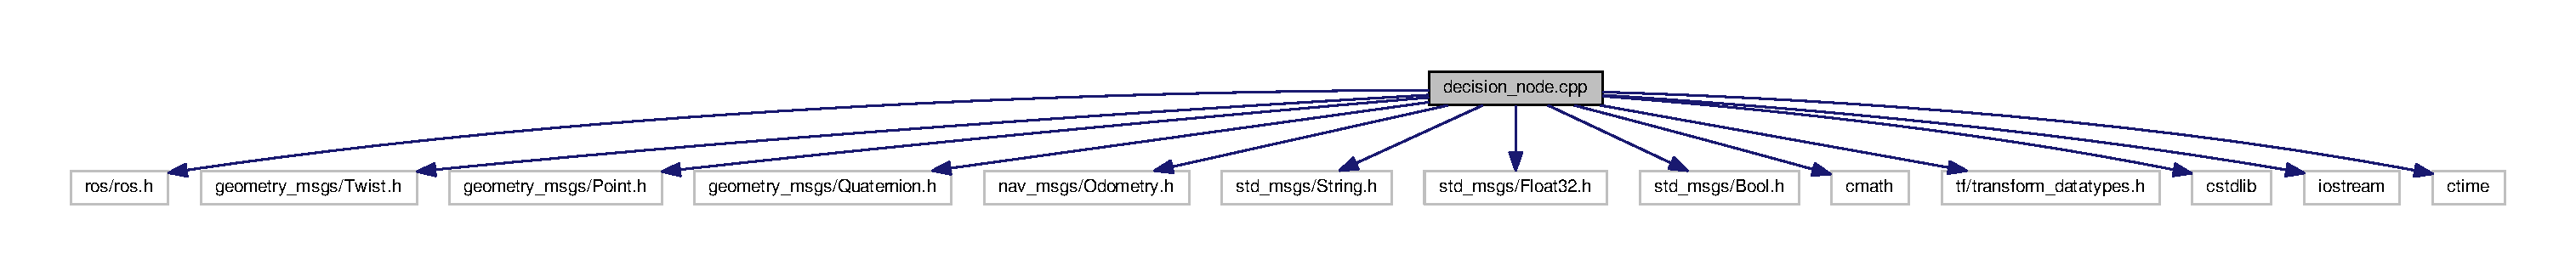
\includegraphics[width=350pt]{decision__node_8cpp__incl}
\end{center}
\end{figure}
\subsection*{Classes}
\begin{DoxyCompactItemize}
\item 
class \hyperlink{classdecision}{decision}
\end{DoxyCompactItemize}
\subsection*{Functions}
\begin{DoxyCompactItemize}
\item 
int {\bfseries main} (int argc, char $\ast$$\ast$argv)\hypertarget{decision__node_8cpp_a3c04138a5bfe5d72780bb7e82a18e627}{}\label{decision__node_8cpp_a3c04138a5bfe5d72780bb7e82a18e627}

\end{DoxyCompactItemize}


\subsection{Detailed Description}
Noeud de décision. 

\begin{DoxyAuthor}{Author}
Groupe 7 
\end{DoxyAuthor}

\hypertarget{obstacle__detection__node_8cpp}{}\section{Référence du fichier obstacle\+\_\+detection\+\_\+node.\+cpp}
\label{obstacle__detection__node_8cpp}\index{obstacle\+\_\+detection\+\_\+node.\+cpp@{obstacle\+\_\+detection\+\_\+node.\+cpp}}


Noeud pour la détection des obstacle  O.\+Aycard.  


{\ttfamily \#include $<$signal.\+h$>$}\\*
{\ttfamily \#include \char`\"{}ros/ros.\+h\char`\"{}}\\*
{\ttfamily \#include \char`\"{}sensor\+\_\+msgs/\+Laser\+Scan.\+h\char`\"{}}\\*
{\ttfamily \#include \char`\"{}visualization\+\_\+msgs/\+Marker.\+h\char`\"{}}\\*
{\ttfamily \#include \char`\"{}geometry\+\_\+msgs/\+Point.\+h\char`\"{}}\\*
{\ttfamily \#include \char`\"{}std\+\_\+msgs/\+Color\+R\+G\+B\+A.\+h\char`\"{}}\\*
{\ttfamily \#include \char`\"{}std\+\_\+msgs/\+Float32.\+h\char`\"{}}\\*
{\ttfamily \#include \char`\"{}std\+\_\+msgs/\+Int32.\+h\char`\"{}}\\*
{\ttfamily \#include $<$cmath$>$}\\*
{\ttfamily \#include \char`\"{}nav\+\_\+msgs/\+Odometry.\+h\char`\"{}}\\*
{\ttfamily \#include $<$tf/transform\+\_\+datatypes.\+h$>$}\\*
{\ttfamily \#include $<$tf/transform\+\_\+listener.\+h$>$}\\*
{\ttfamily \#include \char`\"{}std\+\_\+srvs/\+Empty.\+h\char`\"{}}\\*
{\ttfamily \#include \char`\"{}tf/transform\+\_\+broadcaster.\+h\char`\"{}}\\*
{\ttfamily \#include \char`\"{}message\+\_\+filters/subscriber.\+h\char`\"{}}\\*
{\ttfamily \#include \char`\"{}tf/message\+\_\+filter.\+h\char`\"{}}\\*
Graphe des dépendances par inclusion de obstacle\+\_\+detection\+\_\+node.\+cpp\+:\nopagebreak
\begin{figure}[H]
\begin{center}
\leavevmode
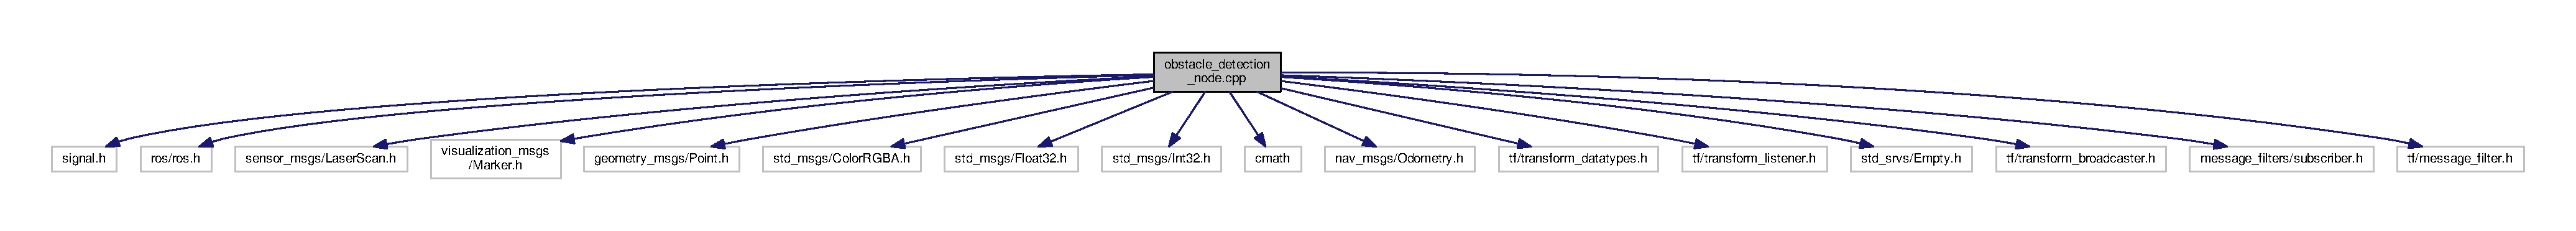
\includegraphics[width=350pt]{obstacle__detection__node_8cpp__incl}
\end{center}
\end{figure}
\subsection*{Classes}
\begin{DoxyCompactItemize}
\item 
class \hyperlink{classobstacle__detection}{obstacle\+\_\+detection}
\begin{DoxyCompactList}\small\item\em Dètecte les obstacle. \end{DoxyCompactList}\end{DoxyCompactItemize}
\subsection*{Fonctions}
\begin{DoxyCompactItemize}
\item 
int \hyperlink{obstacle__detection__node_8cpp_a3c04138a5bfe5d72780bb7e82a18e627}{main} (int argc, char $\ast$$\ast$argv)
\end{DoxyCompactItemize}
\subsection*{Variables}
\begin{DoxyCompactItemize}
\item 
float \hyperlink{obstacle__detection__node_8cpp_af22d0c09c0f6f6b9c486b2a90867d7e6}{robair\+\_\+size} = 0.\+2
\end{DoxyCompactItemize}


\subsection{Description détaillée}
Noeud pour la détection des obstacle  O.\+Aycard. 



\subsection{Documentation des fonctions}
\index{obstacle\+\_\+detection\+\_\+node.\+cpp@{obstacle\+\_\+detection\+\_\+node.\+cpp}!main@{main}}
\index{main@{main}!obstacle\+\_\+detection\+\_\+node.\+cpp@{obstacle\+\_\+detection\+\_\+node.\+cpp}}
\subsubsection[{\texorpdfstring{main(int argc, char $\ast$$\ast$argv)}{main(int argc, char **argv)}}]{\setlength{\rightskip}{0pt plus 5cm}int main (
\begin{DoxyParamCaption}
\item[{int}]{argc, }
\item[{char $\ast$$\ast$}]{argv}
\end{DoxyParamCaption}
)}\hypertarget{obstacle__detection__node_8cpp_a3c04138a5bfe5d72780bb7e82a18e627}{}\label{obstacle__detection__node_8cpp_a3c04138a5bfe5d72780bb7e82a18e627}


\subsection{Documentation des variables}
\index{obstacle\+\_\+detection\+\_\+node.\+cpp@{obstacle\+\_\+detection\+\_\+node.\+cpp}!robair\+\_\+size@{robair\+\_\+size}}
\index{robair\+\_\+size@{robair\+\_\+size}!obstacle\+\_\+detection\+\_\+node.\+cpp@{obstacle\+\_\+detection\+\_\+node.\+cpp}}
\subsubsection[{\texorpdfstring{robair\+\_\+size}{robair_size}}]{\setlength{\rightskip}{0pt plus 5cm}float robair\+\_\+size = 0.\+2}\hypertarget{obstacle__detection__node_8cpp_af22d0c09c0f6f6b9c486b2a90867d7e6}{}\label{obstacle__detection__node_8cpp_af22d0c09c0f6f6b9c486b2a90867d7e6}

\hypertarget{persons__detection__node_8cpp}{}\section{Référence du fichier persons\+\_\+detection\+\_\+node.\+cpp}
\label{persons__detection__node_8cpp}\index{persons\+\_\+detection\+\_\+node.\+cpp@{persons\+\_\+detection\+\_\+node.\+cpp}}


Neud pour la détection de personnes  Groupe 7.  


{\ttfamily \#include \char`\"{}ros/ros.\+h\char`\"{}}\\*
{\ttfamily \#include \char`\"{}ros/time.\+h\char`\"{}}\\*
{\ttfamily \#include \char`\"{}sensor\+\_\+msgs/\+Laser\+Scan.\+h\char`\"{}}\\*
{\ttfamily \#include \char`\"{}visualization\+\_\+msgs/\+Marker.\+h\char`\"{}}\\*
{\ttfamily \#include \char`\"{}geometry\+\_\+msgs/\+Point.\+h\char`\"{}}\\*
{\ttfamily \#include \char`\"{}geometry\+\_\+msgs/\+Pose\+Array.\+h\char`\"{}}\\*
{\ttfamily \#include \char`\"{}geometry\+\_\+msgs/\+Pose.\+h\char`\"{}}\\*
{\ttfamily \#include \char`\"{}std\+\_\+msgs/\+Color\+R\+G\+B\+A.\+h\char`\"{}}\\*
{\ttfamily \#include $<$cmath$>$}\\*
{\ttfamily \#include \char`\"{}std\+\_\+msgs/\+Bool.\+h\char`\"{}}\\*
Graphe des dépendances par inclusion de persons\+\_\+detection\+\_\+node.\+cpp\+:\nopagebreak
\begin{figure}[H]
\begin{center}
\leavevmode
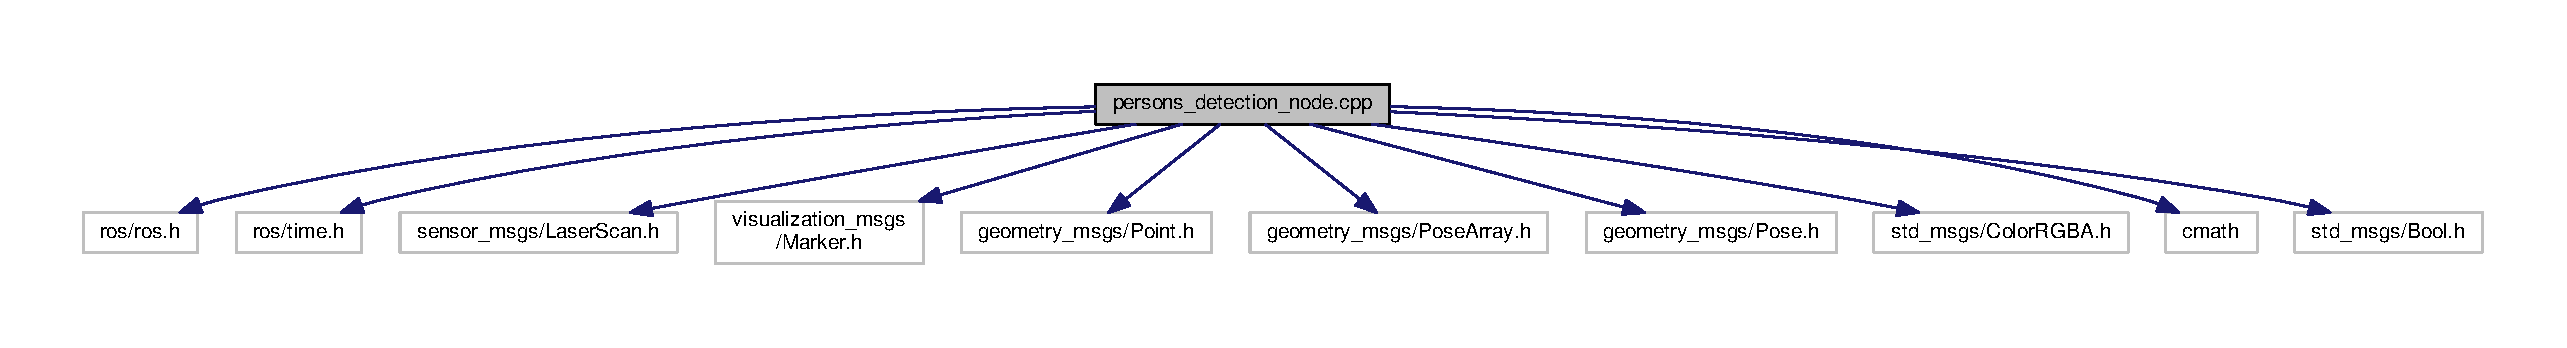
\includegraphics[width=350pt]{persons__detection__node_8cpp__incl}
\end{center}
\end{figure}
\subsection*{Classes}
\begin{DoxyCompactItemize}
\item 
class \hyperlink{classmoving__persons__detector}{moving\+\_\+persons\+\_\+detector}
\begin{DoxyCompactList}\small\item\em Détecte les personnes et les groupes. \end{DoxyCompactList}\end{DoxyCompactItemize}
\subsection*{Macros}
\begin{DoxyCompactItemize}
\item 
\#define \hyperlink{persons__detection__node_8cpp_a709da7b9e1c2848cb6c69a545c6e05d0}{cluster\+\_\+threshold}~0.\+2
\item 
\#define \hyperlink{persons__detection__node_8cpp_ae6095eddd47a8cb26f5b45e49187bb02}{detection\+\_\+threshold}~0.\+2
\item 
\#define \hyperlink{persons__detection__node_8cpp_a92dbe0db25628989b794cc93b67e1571}{dynamic\+\_\+threshold}~0
\item 
\#define \hyperlink{persons__detection__node_8cpp_aa2fdb1ea3da051bb30fe1edb9951e889}{group\+\_\+person\+\_\+threshold}~0.\+8
\item 
\#define \hyperlink{persons__detection__node_8cpp_a3966a6eabc388975b51acf5f6e4ad235}{leg\+\_\+size\+\_\+min}~0.\+1
\item 
\#define \hyperlink{persons__detection__node_8cpp_a72777780f3427bf299bbec7640b6cb1a}{leg\+\_\+size\+\_\+max}~0.\+3
\item 
\#define \hyperlink{persons__detection__node_8cpp_a68fa36224acb098fe17c1324ceda84d6}{legs\+\_\+distance\+\_\+max}~1
\item 
\#define \hyperlink{persons__detection__node_8cpp_aeb857e941c056f14dc583d14be995c10}{distance\+\_\+person}~1.\+5
\item 
\#define \hyperlink{persons__detection__node_8cpp_a00809aad6f43c127152f5b0f32776402}{iter\+\_\+person}~10
\item 
\#define \hyperlink{persons__detection__node_8cpp_a1313c948b75a0a0cfb0fad8334bc1d13}{min\+\_\+view}~7
\end{DoxyCompactItemize}
\subsection*{Fonctions}
\begin{DoxyCompactItemize}
\item 
int \hyperlink{persons__detection__node_8cpp_a3c04138a5bfe5d72780bb7e82a18e627}{main} (int argc, char $\ast$$\ast$argv)
\end{DoxyCompactItemize}


\subsection{Description détaillée}
Neud pour la détection de personnes  Groupe 7. 



\subsection{Documentation des macros}
\index{persons\+\_\+detection\+\_\+node.\+cpp@{persons\+\_\+detection\+\_\+node.\+cpp}!cluster\+\_\+threshold@{cluster\+\_\+threshold}}
\index{cluster\+\_\+threshold@{cluster\+\_\+threshold}!persons\+\_\+detection\+\_\+node.\+cpp@{persons\+\_\+detection\+\_\+node.\+cpp}}
\subsubsection[{\texorpdfstring{cluster\+\_\+threshold}{cluster_threshold}}]{\setlength{\rightskip}{0pt plus 5cm}\#define cluster\+\_\+threshold~0.\+2}\hypertarget{persons__detection__node_8cpp_a709da7b9e1c2848cb6c69a545c6e05d0}{}\label{persons__detection__node_8cpp_a709da7b9e1c2848cb6c69a545c6e05d0}
Distance entre deux points pour qu\textquotesingle{}ils appartiennent au même cluster \index{persons\+\_\+detection\+\_\+node.\+cpp@{persons\+\_\+detection\+\_\+node.\+cpp}!detection\+\_\+threshold@{detection\+\_\+threshold}}
\index{detection\+\_\+threshold@{detection\+\_\+threshold}!persons\+\_\+detection\+\_\+node.\+cpp@{persons\+\_\+detection\+\_\+node.\+cpp}}
\subsubsection[{\texorpdfstring{detection\+\_\+threshold}{detection_threshold}}]{\setlength{\rightskip}{0pt plus 5cm}\#define detection\+\_\+threshold~0.\+2}\hypertarget{persons__detection__node_8cpp_ae6095eddd47a8cb26f5b45e49187bb02}{}\label{persons__detection__node_8cpp_ae6095eddd47a8cb26f5b45e49187bb02}
\index{persons\+\_\+detection\+\_\+node.\+cpp@{persons\+\_\+detection\+\_\+node.\+cpp}!distance\+\_\+person@{distance\+\_\+person}}
\index{distance\+\_\+person@{distance\+\_\+person}!persons\+\_\+detection\+\_\+node.\+cpp@{persons\+\_\+detection\+\_\+node.\+cpp}}
\subsubsection[{\texorpdfstring{distance\+\_\+person}{distance_person}}]{\setlength{\rightskip}{0pt plus 5cm}\#define distance\+\_\+person~1.\+5}\hypertarget{persons__detection__node_8cpp_aeb857e941c056f14dc583d14be995c10}{}\label{persons__detection__node_8cpp_aeb857e941c056f14dc583d14be995c10}
Distance maximale entre deux personnes d\textquotesingle{}un même groupe \index{persons\+\_\+detection\+\_\+node.\+cpp@{persons\+\_\+detection\+\_\+node.\+cpp}!dynamic\+\_\+threshold@{dynamic\+\_\+threshold}}
\index{dynamic\+\_\+threshold@{dynamic\+\_\+threshold}!persons\+\_\+detection\+\_\+node.\+cpp@{persons\+\_\+detection\+\_\+node.\+cpp}}
\subsubsection[{\texorpdfstring{dynamic\+\_\+threshold}{dynamic_threshold}}]{\setlength{\rightskip}{0pt plus 5cm}\#define dynamic\+\_\+threshold~0}\hypertarget{persons__detection__node_8cpp_a92dbe0db25628989b794cc93b67e1571}{}\label{persons__detection__node_8cpp_a92dbe0db25628989b794cc93b67e1571}
Taux de points dynamique \index{persons\+\_\+detection\+\_\+node.\+cpp@{persons\+\_\+detection\+\_\+node.\+cpp}!group\+\_\+person\+\_\+threshold@{group\+\_\+person\+\_\+threshold}}
\index{group\+\_\+person\+\_\+threshold@{group\+\_\+person\+\_\+threshold}!persons\+\_\+detection\+\_\+node.\+cpp@{persons\+\_\+detection\+\_\+node.\+cpp}}
\subsubsection[{\texorpdfstring{group\+\_\+person\+\_\+threshold}{group_person_threshold}}]{\setlength{\rightskip}{0pt plus 5cm}\#define group\+\_\+person\+\_\+threshold~0.\+8}\hypertarget{persons__detection__node_8cpp_aa2fdb1ea3da051bb30fe1edb9951e889}{}\label{persons__detection__node_8cpp_aa2fdb1ea3da051bb30fe1edb9951e889}
\index{persons\+\_\+detection\+\_\+node.\+cpp@{persons\+\_\+detection\+\_\+node.\+cpp}!iter\+\_\+person@{iter\+\_\+person}}
\index{iter\+\_\+person@{iter\+\_\+person}!persons\+\_\+detection\+\_\+node.\+cpp@{persons\+\_\+detection\+\_\+node.\+cpp}}
\subsubsection[{\texorpdfstring{iter\+\_\+person}{iter_person}}]{\setlength{\rightskip}{0pt plus 5cm}\#define iter\+\_\+person~10}\hypertarget{persons__detection__node_8cpp_a00809aad6f43c127152f5b0f32776402}{}\label{persons__detection__node_8cpp_a00809aad6f43c127152f5b0f32776402}
Nombre d\textquotesingle{}iteration pour la détection \index{persons\+\_\+detection\+\_\+node.\+cpp@{persons\+\_\+detection\+\_\+node.\+cpp}!leg\+\_\+size\+\_\+max@{leg\+\_\+size\+\_\+max}}
\index{leg\+\_\+size\+\_\+max@{leg\+\_\+size\+\_\+max}!persons\+\_\+detection\+\_\+node.\+cpp@{persons\+\_\+detection\+\_\+node.\+cpp}}
\subsubsection[{\texorpdfstring{leg\+\_\+size\+\_\+max}{leg_size_max}}]{\setlength{\rightskip}{0pt plus 5cm}\#define leg\+\_\+size\+\_\+max~0.\+3}\hypertarget{persons__detection__node_8cpp_a72777780f3427bf299bbec7640b6cb1a}{}\label{persons__detection__node_8cpp_a72777780f3427bf299bbec7640b6cb1a}
Largeur maximale d\textquotesingle{}une jambe \index{persons\+\_\+detection\+\_\+node.\+cpp@{persons\+\_\+detection\+\_\+node.\+cpp}!leg\+\_\+size\+\_\+min@{leg\+\_\+size\+\_\+min}}
\index{leg\+\_\+size\+\_\+min@{leg\+\_\+size\+\_\+min}!persons\+\_\+detection\+\_\+node.\+cpp@{persons\+\_\+detection\+\_\+node.\+cpp}}
\subsubsection[{\texorpdfstring{leg\+\_\+size\+\_\+min}{leg_size_min}}]{\setlength{\rightskip}{0pt plus 5cm}\#define leg\+\_\+size\+\_\+min~0.\+1}\hypertarget{persons__detection__node_8cpp_a3966a6eabc388975b51acf5f6e4ad235}{}\label{persons__detection__node_8cpp_a3966a6eabc388975b51acf5f6e4ad235}
Largeur minimale d\textquotesingle{}une jambe \index{persons\+\_\+detection\+\_\+node.\+cpp@{persons\+\_\+detection\+\_\+node.\+cpp}!legs\+\_\+distance\+\_\+max@{legs\+\_\+distance\+\_\+max}}
\index{legs\+\_\+distance\+\_\+max@{legs\+\_\+distance\+\_\+max}!persons\+\_\+detection\+\_\+node.\+cpp@{persons\+\_\+detection\+\_\+node.\+cpp}}
\subsubsection[{\texorpdfstring{legs\+\_\+distance\+\_\+max}{legs_distance_max}}]{\setlength{\rightskip}{0pt plus 5cm}\#define legs\+\_\+distance\+\_\+max~1}\hypertarget{persons__detection__node_8cpp_a68fa36224acb098fe17c1324ceda84d6}{}\label{persons__detection__node_8cpp_a68fa36224acb098fe17c1324ceda84d6}
Distance maximale entre deux jambes d\textquotesingle{}une personne \index{persons\+\_\+detection\+\_\+node.\+cpp@{persons\+\_\+detection\+\_\+node.\+cpp}!min\+\_\+view@{min\+\_\+view}}
\index{min\+\_\+view@{min\+\_\+view}!persons\+\_\+detection\+\_\+node.\+cpp@{persons\+\_\+detection\+\_\+node.\+cpp}}
\subsubsection[{\texorpdfstring{min\+\_\+view}{min_view}}]{\setlength{\rightskip}{0pt plus 5cm}\#define min\+\_\+view~7}\hypertarget{persons__detection__node_8cpp_a1313c948b75a0a0cfb0fad8334bc1d13}{}\label{persons__detection__node_8cpp_a1313c948b75a0a0cfb0fad8334bc1d13}
Nombre de vue minimum pour la détection 

\subsection{Documentation des fonctions}
\index{persons\+\_\+detection\+\_\+node.\+cpp@{persons\+\_\+detection\+\_\+node.\+cpp}!main@{main}}
\index{main@{main}!persons\+\_\+detection\+\_\+node.\+cpp@{persons\+\_\+detection\+\_\+node.\+cpp}}
\subsubsection[{\texorpdfstring{main(int argc, char $\ast$$\ast$argv)}{main(int argc, char **argv)}}]{\setlength{\rightskip}{0pt plus 5cm}int main (
\begin{DoxyParamCaption}
\item[{int}]{argc, }
\item[{char $\ast$$\ast$}]{argv}
\end{DoxyParamCaption}
)}\hypertarget{persons__detection__node_8cpp_a3c04138a5bfe5d72780bb7e82a18e627}{}\label{persons__detection__node_8cpp_a3c04138a5bfe5d72780bb7e82a18e627}

\hypertarget{robot__moving__node_8cpp}{}\section{Référence du fichier robot\+\_\+moving\+\_\+node.\+cpp}
\label{robot__moving__node_8cpp}\index{robot\+\_\+moving\+\_\+node.\+cpp@{robot\+\_\+moving\+\_\+node.\+cpp}}


Détect les ouvement du robot  O.\+Aycard.  


{\ttfamily \#include $<$signal.\+h$>$}\\*
{\ttfamily \#include \char`\"{}ros/ros.\+h\char`\"{}}\\*
{\ttfamily \#include \char`\"{}sensor\+\_\+msgs/\+Laser\+Scan.\+h\char`\"{}}\\*
{\ttfamily \#include \char`\"{}visualization\+\_\+msgs/\+Marker.\+h\char`\"{}}\\*
{\ttfamily \#include \char`\"{}geometry\+\_\+msgs/\+Point.\+h\char`\"{}}\\*
{\ttfamily \#include \char`\"{}std\+\_\+msgs/\+Color\+R\+G\+B\+A.\+h\char`\"{}}\\*
{\ttfamily \#include \char`\"{}std\+\_\+msgs/\+Float32.\+h\char`\"{}}\\*
{\ttfamily \#include \char`\"{}std\+\_\+msgs/\+Bool.\+h\char`\"{}}\\*
{\ttfamily \#include $<$cmath$>$}\\*
{\ttfamily \#include \char`\"{}nav\+\_\+msgs/\+Odometry.\+h\char`\"{}}\\*
{\ttfamily \#include $<$tf/transform\+\_\+datatypes.\+h$>$}\\*
{\ttfamily \#include $<$tf/transform\+\_\+listener.\+h$>$}\\*
{\ttfamily \#include \char`\"{}std\+\_\+srvs/\+Empty.\+h\char`\"{}}\\*
{\ttfamily \#include \char`\"{}tf/transform\+\_\+broadcaster.\+h\char`\"{}}\\*
{\ttfamily \#include \char`\"{}message\+\_\+filters/subscriber.\+h\char`\"{}}\\*
{\ttfamily \#include \char`\"{}tf/message\+\_\+filter.\+h\char`\"{}}\\*
Graphe des dépendances par inclusion de robot\+\_\+moving\+\_\+node.\+cpp\+:\nopagebreak
\begin{figure}[H]
\begin{center}
\leavevmode
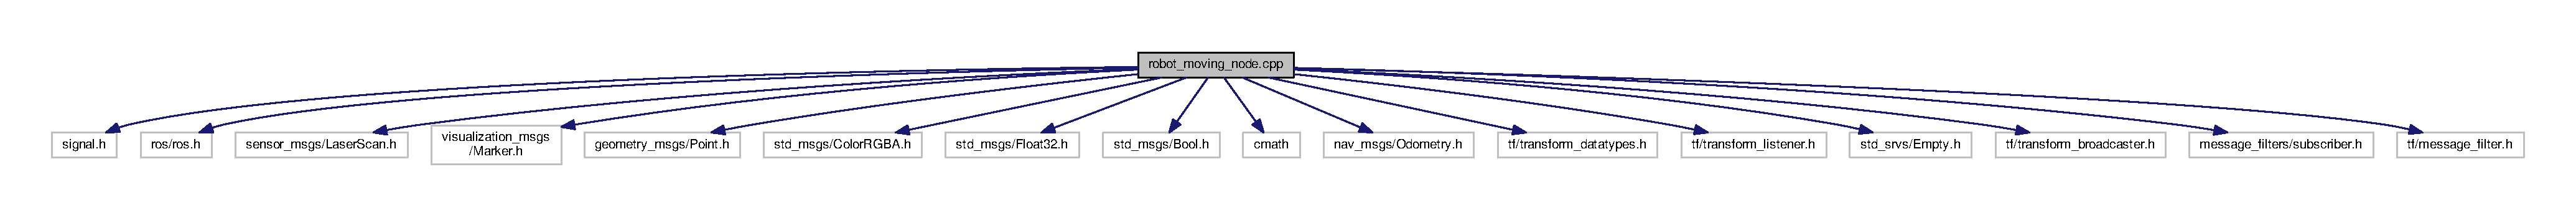
\includegraphics[width=350pt]{robot__moving__node_8cpp__incl}
\end{center}
\end{figure}
\subsection*{Classes}
\begin{DoxyCompactItemize}
\item 
class \hyperlink{classrobot__moving__lectures}{robot\+\_\+moving\+\_\+lectures}
\begin{DoxyCompactList}\small\item\em Vérifie que le robot est en mouvement. \end{DoxyCompactList}\end{DoxyCompactItemize}
\subsection*{Fonctions}
\begin{DoxyCompactItemize}
\item 
int \hyperlink{robot__moving__node_8cpp_a3c04138a5bfe5d72780bb7e82a18e627}{main} (int argc, char $\ast$$\ast$argv)
\end{DoxyCompactItemize}
\subsection*{Variables}
\begin{DoxyCompactItemize}
\item 
int \hyperlink{robot__moving__node_8cpp_aa5218da2c57837e43c73faa2fef3ea67}{nb\+\_\+static} = 5
\end{DoxyCompactItemize}


\subsection{Description détaillée}
Détect les ouvement du robot  O.\+Aycard. 



\subsection{Documentation des fonctions}
\index{robot\+\_\+moving\+\_\+node.\+cpp@{robot\+\_\+moving\+\_\+node.\+cpp}!main@{main}}
\index{main@{main}!robot\+\_\+moving\+\_\+node.\+cpp@{robot\+\_\+moving\+\_\+node.\+cpp}}
\subsubsection[{\texorpdfstring{main(int argc, char $\ast$$\ast$argv)}{main(int argc, char **argv)}}]{\setlength{\rightskip}{0pt plus 5cm}int main (
\begin{DoxyParamCaption}
\item[{int}]{argc, }
\item[{char $\ast$$\ast$}]{argv}
\end{DoxyParamCaption}
)}\hypertarget{robot__moving__node_8cpp_a3c04138a5bfe5d72780bb7e82a18e627}{}\label{robot__moving__node_8cpp_a3c04138a5bfe5d72780bb7e82a18e627}


\subsection{Documentation des variables}
\index{robot\+\_\+moving\+\_\+node.\+cpp@{robot\+\_\+moving\+\_\+node.\+cpp}!nb\+\_\+static@{nb\+\_\+static}}
\index{nb\+\_\+static@{nb\+\_\+static}!robot\+\_\+moving\+\_\+node.\+cpp@{robot\+\_\+moving\+\_\+node.\+cpp}}
\subsubsection[{\texorpdfstring{nb\+\_\+static}{nb_static}}]{\setlength{\rightskip}{0pt plus 5cm}int nb\+\_\+static = 5}\hypertarget{robot__moving__node_8cpp_aa5218da2c57837e43c73faa2fef3ea67}{}\label{robot__moving__node_8cpp_aa5218da2c57837e43c73faa2fef3ea67}

\hypertarget{rotation__action__node_8cpp}{}\section{Référence du fichier rotation\+\_\+action\+\_\+node.\+cpp}
\label{rotation__action__node_8cpp}\index{rotation\+\_\+action\+\_\+node.\+cpp@{rotation\+\_\+action\+\_\+node.\+cpp}}


Noeud pour effectuer des translation  O.\+Aycard.  


{\ttfamily \#include \char`\"{}ros/ros.\+h\char`\"{}}\\*
{\ttfamily \#include $<$geometry\+\_\+msgs/\+Twist.\+h$>$}\\*
{\ttfamily \#include \char`\"{}geometry\+\_\+msgs/\+Point.\+h\char`\"{}}\\*
{\ttfamily \#include \char`\"{}geometry\+\_\+msgs/\+Quaternion.\+h\char`\"{}}\\*
{\ttfamily \#include \char`\"{}nav\+\_\+msgs/\+Odometry.\+h\char`\"{}}\\*
{\ttfamily \#include \char`\"{}std\+\_\+msgs/\+String.\+h\char`\"{}}\\*
{\ttfamily \#include \char`\"{}std\+\_\+msgs/\+Float32.\+h\char`\"{}}\\*
{\ttfamily \#include $<$cmath$>$}\\*
{\ttfamily \#include $<$tf/transform\+\_\+datatypes.\+h$>$}\\*
Graphe des dépendances par inclusion de rotation\+\_\+action\+\_\+node.\+cpp\+:\nopagebreak
\begin{figure}[H]
\begin{center}
\leavevmode
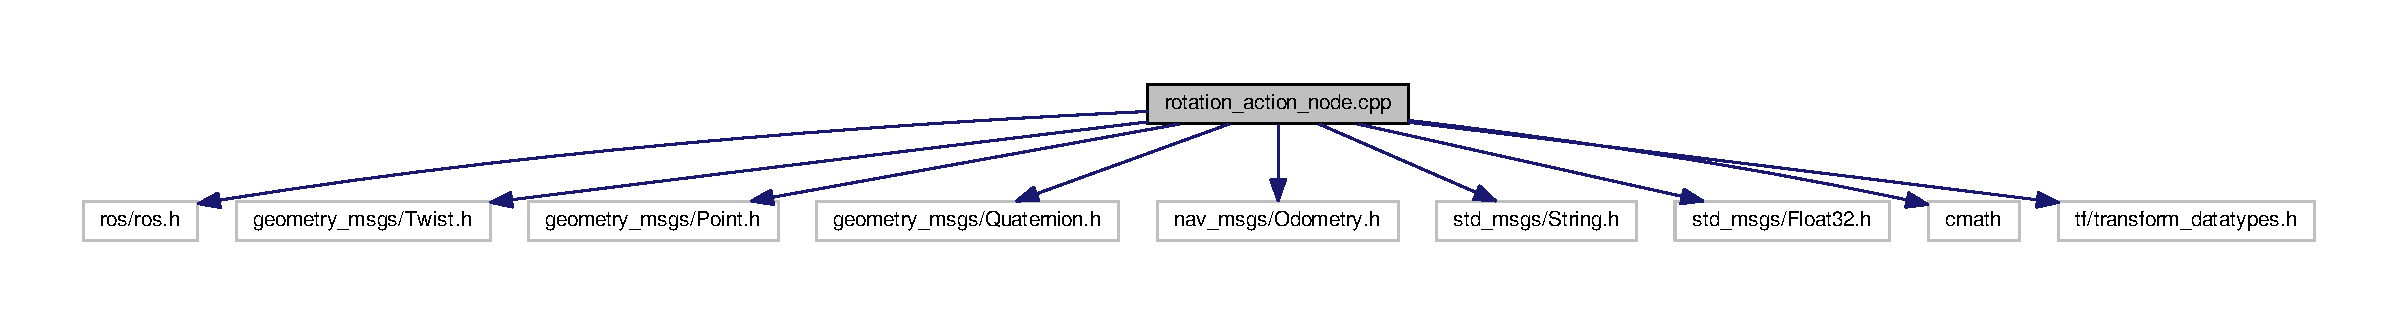
\includegraphics[width=350pt]{rotation__action__node_8cpp__incl}
\end{center}
\end{figure}
\subsection*{Classes}
\begin{DoxyCompactItemize}
\item 
class \hyperlink{classrotation__action}{rotation\+\_\+action}
\begin{DoxyCompactList}\small\item\em Gère la rotation du robot. \end{DoxyCompactList}\end{DoxyCompactItemize}
\subsection*{Macros}
\begin{DoxyCompactItemize}
\item 
\#define \hyperlink{rotation__action__node_8cpp_aac72bea45fe64e877f39a9f3af7f56b5}{rotation\+\_\+error}~0.\+2
\item 
\#define \hyperlink{rotation__action__node_8cpp_a4a22f30a94d579ec099493eaa3e3cfec}{kp}~0.\+5
\item 
\#define \hyperlink{rotation__action__node_8cpp_ac208d4a15168228961f22ff0619bd468}{ki}~0
\item 
\#define \hyperlink{rotation__action__node_8cpp_a731039d1eebab67f74b726ab9aec55a6}{kd}~0
\end{DoxyCompactItemize}
\subsection*{Fonctions}
\begin{DoxyCompactItemize}
\item 
int \hyperlink{rotation__action__node_8cpp_a3c04138a5bfe5d72780bb7e82a18e627}{main} (int argc, char $\ast$$\ast$argv)
\end{DoxyCompactItemize}


\subsection{Description détaillée}
Noeud pour effectuer des translation  O.\+Aycard. 



\subsection{Documentation des macros}
\index{rotation\+\_\+action\+\_\+node.\+cpp@{rotation\+\_\+action\+\_\+node.\+cpp}!kd@{kd}}
\index{kd@{kd}!rotation\+\_\+action\+\_\+node.\+cpp@{rotation\+\_\+action\+\_\+node.\+cpp}}
\subsubsection[{\texorpdfstring{kd}{kd}}]{\setlength{\rightskip}{0pt plus 5cm}\#define kd~0}\hypertarget{rotation__action__node_8cpp_a731039d1eebab67f74b726ab9aec55a6}{}\label{rotation__action__node_8cpp_a731039d1eebab67f74b726ab9aec55a6}
coefficient kd \index{rotation\+\_\+action\+\_\+node.\+cpp@{rotation\+\_\+action\+\_\+node.\+cpp}!ki@{ki}}
\index{ki@{ki}!rotation\+\_\+action\+\_\+node.\+cpp@{rotation\+\_\+action\+\_\+node.\+cpp}}
\subsubsection[{\texorpdfstring{ki}{ki}}]{\setlength{\rightskip}{0pt plus 5cm}\#define ki~0}\hypertarget{rotation__action__node_8cpp_ac208d4a15168228961f22ff0619bd468}{}\label{rotation__action__node_8cpp_ac208d4a15168228961f22ff0619bd468}
coefficient ki \index{rotation\+\_\+action\+\_\+node.\+cpp@{rotation\+\_\+action\+\_\+node.\+cpp}!kp@{kp}}
\index{kp@{kp}!rotation\+\_\+action\+\_\+node.\+cpp@{rotation\+\_\+action\+\_\+node.\+cpp}}
\subsubsection[{\texorpdfstring{kp}{kp}}]{\setlength{\rightskip}{0pt plus 5cm}\#define kp~0.\+5}\hypertarget{rotation__action__node_8cpp_a4a22f30a94d579ec099493eaa3e3cfec}{}\label{rotation__action__node_8cpp_a4a22f30a94d579ec099493eaa3e3cfec}
coefficient kp \index{rotation\+\_\+action\+\_\+node.\+cpp@{rotation\+\_\+action\+\_\+node.\+cpp}!rotation\+\_\+error@{rotation\+\_\+error}}
\index{rotation\+\_\+error@{rotation\+\_\+error}!rotation\+\_\+action\+\_\+node.\+cpp@{rotation\+\_\+action\+\_\+node.\+cpp}}
\subsubsection[{\texorpdfstring{rotation\+\_\+error}{rotation_error}}]{\setlength{\rightskip}{0pt plus 5cm}\#define rotation\+\_\+error~0.\+2}\hypertarget{rotation__action__node_8cpp_aac72bea45fe64e877f39a9f3af7f56b5}{}\label{rotation__action__node_8cpp_aac72bea45fe64e877f39a9f3af7f56b5}
Erreur pour la rotation 

\subsection{Documentation des fonctions}
\index{rotation\+\_\+action\+\_\+node.\+cpp@{rotation\+\_\+action\+\_\+node.\+cpp}!main@{main}}
\index{main@{main}!rotation\+\_\+action\+\_\+node.\+cpp@{rotation\+\_\+action\+\_\+node.\+cpp}}
\subsubsection[{\texorpdfstring{main(int argc, char $\ast$$\ast$argv)}{main(int argc, char **argv)}}]{\setlength{\rightskip}{0pt plus 5cm}int main (
\begin{DoxyParamCaption}
\item[{int}]{argc, }
\item[{char $\ast$$\ast$}]{argv}
\end{DoxyParamCaption}
)}\hypertarget{rotation__action__node_8cpp_a3c04138a5bfe5d72780bb7e82a18e627}{}\label{rotation__action__node_8cpp_a3c04138a5bfe5d72780bb7e82a18e627}

\hypertarget{translation__action__node_8cpp}{}\section{Référence du fichier translation\+\_\+action\+\_\+node.\+cpp}
\label{translation__action__node_8cpp}\index{translation\+\_\+action\+\_\+node.\+cpp@{translation\+\_\+action\+\_\+node.\+cpp}}


Noeud pour effectuer des translation  O.\+Aycard.  


{\ttfamily \#include \char`\"{}ros/ros.\+h\char`\"{}}\\*
{\ttfamily \#include \char`\"{}sensor\+\_\+msgs/\+Laser\+Scan.\+h\char`\"{}}\\*
{\ttfamily \#include \char`\"{}visualization\+\_\+msgs/\+Marker.\+h\char`\"{}}\\*
{\ttfamily \#include \char`\"{}geometry\+\_\+msgs/\+Point.\+h\char`\"{}}\\*
{\ttfamily \#include \char`\"{}std\+\_\+msgs/\+Color\+R\+G\+B\+A.\+h\char`\"{}}\\*
{\ttfamily \#include \char`\"{}std\+\_\+msgs/\+Float32.\+h\char`\"{}}\\*
{\ttfamily \#include $<$cmath$>$}\\*
{\ttfamily \#include \char`\"{}nav\+\_\+msgs/\+Odometry.\+h\char`\"{}}\\*
{\ttfamily \#include $<$tf/transform\+\_\+datatypes.\+h$>$}\\*
Graphe des dépendances par inclusion de translation\+\_\+action\+\_\+node.\+cpp\+:\nopagebreak
\begin{figure}[H]
\begin{center}
\leavevmode
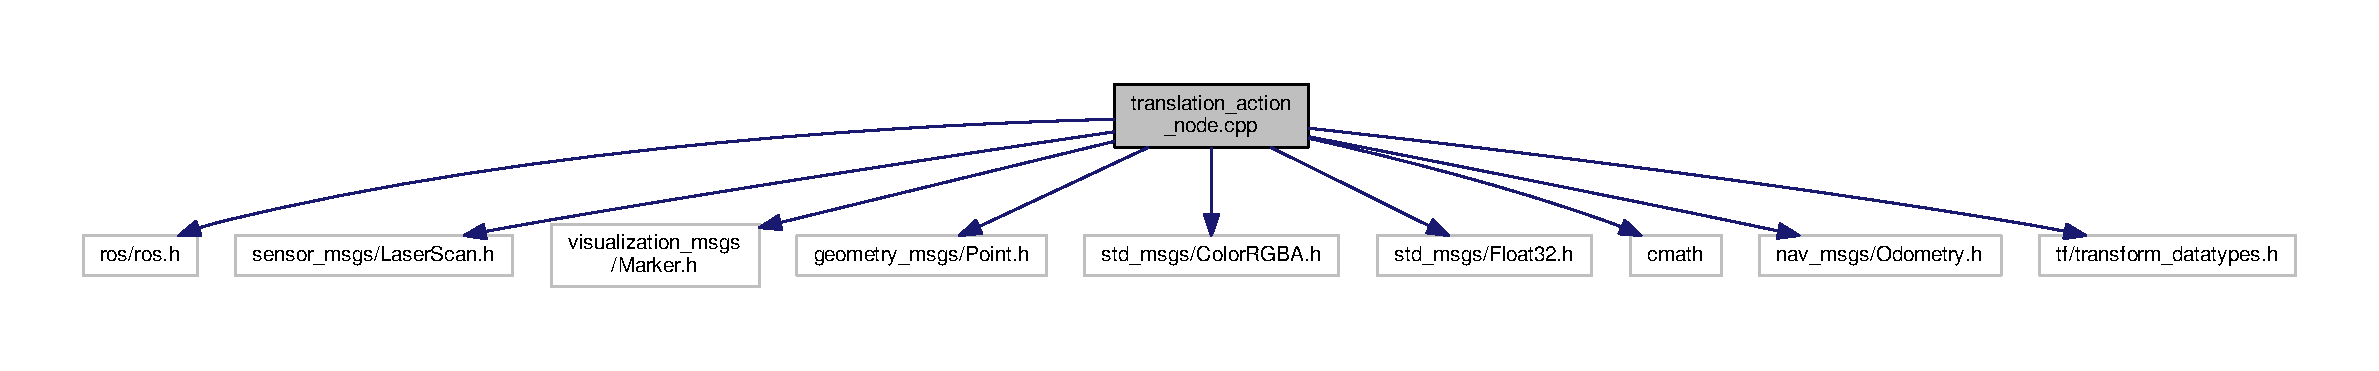
\includegraphics[width=350pt]{translation__action__node_8cpp__incl}
\end{center}
\end{figure}
\subsection*{Classes}
\begin{DoxyCompactItemize}
\item 
class \hyperlink{classtranslation__action}{translation\+\_\+action}
\begin{DoxyCompactList}\small\item\em Gère les translations du robot. \end{DoxyCompactList}\end{DoxyCompactItemize}
\subsection*{Macros}
\begin{DoxyCompactItemize}
\item 
\#define \hyperlink{translation__action__node_8cpp_a4e7b3388a51eede7d0c430d606162c1a}{security\+\_\+distance}~0.\+5
\item 
\#define \hyperlink{translation__action__node_8cpp_a1c9b17ecd759bf14bd10c47d68771173}{translation\+\_\+error}~0.\+1
\item 
\#define \hyperlink{translation__action__node_8cpp_a4a22f30a94d579ec099493eaa3e3cfec}{kp}~0.\+5
\item 
\#define \hyperlink{translation__action__node_8cpp_ac208d4a15168228961f22ff0619bd468}{ki}~0
\item 
\#define \hyperlink{translation__action__node_8cpp_a731039d1eebab67f74b726ab9aec55a6}{kd}~0
\end{DoxyCompactItemize}
\subsection*{Fonctions}
\begin{DoxyCompactItemize}
\item 
int \hyperlink{translation__action__node_8cpp_a3c04138a5bfe5d72780bb7e82a18e627}{main} (int argc, char $\ast$$\ast$argv)
\end{DoxyCompactItemize}


\subsection{Description détaillée}
Noeud pour effectuer des translation  O.\+Aycard. 



\subsection{Documentation des macros}
\index{translation\+\_\+action\+\_\+node.\+cpp@{translation\+\_\+action\+\_\+node.\+cpp}!kd@{kd}}
\index{kd@{kd}!translation\+\_\+action\+\_\+node.\+cpp@{translation\+\_\+action\+\_\+node.\+cpp}}
\subsubsection[{\texorpdfstring{kd}{kd}}]{\setlength{\rightskip}{0pt plus 5cm}\#define kd~0}\hypertarget{translation__action__node_8cpp_a731039d1eebab67f74b726ab9aec55a6}{}\label{translation__action__node_8cpp_a731039d1eebab67f74b726ab9aec55a6}
coefficient kd \index{translation\+\_\+action\+\_\+node.\+cpp@{translation\+\_\+action\+\_\+node.\+cpp}!ki@{ki}}
\index{ki@{ki}!translation\+\_\+action\+\_\+node.\+cpp@{translation\+\_\+action\+\_\+node.\+cpp}}
\subsubsection[{\texorpdfstring{ki}{ki}}]{\setlength{\rightskip}{0pt plus 5cm}\#define ki~0}\hypertarget{translation__action__node_8cpp_ac208d4a15168228961f22ff0619bd468}{}\label{translation__action__node_8cpp_ac208d4a15168228961f22ff0619bd468}
coefficient ki \index{translation\+\_\+action\+\_\+node.\+cpp@{translation\+\_\+action\+\_\+node.\+cpp}!kp@{kp}}
\index{kp@{kp}!translation\+\_\+action\+\_\+node.\+cpp@{translation\+\_\+action\+\_\+node.\+cpp}}
\subsubsection[{\texorpdfstring{kp}{kp}}]{\setlength{\rightskip}{0pt plus 5cm}\#define kp~0.\+5}\hypertarget{translation__action__node_8cpp_a4a22f30a94d579ec099493eaa3e3cfec}{}\label{translation__action__node_8cpp_a4a22f30a94d579ec099493eaa3e3cfec}
coefficient kp \index{translation\+\_\+action\+\_\+node.\+cpp@{translation\+\_\+action\+\_\+node.\+cpp}!security\+\_\+distance@{security\+\_\+distance}}
\index{security\+\_\+distance@{security\+\_\+distance}!translation\+\_\+action\+\_\+node.\+cpp@{translation\+\_\+action\+\_\+node.\+cpp}}
\subsubsection[{\texorpdfstring{security\+\_\+distance}{security_distance}}]{\setlength{\rightskip}{0pt plus 5cm}\#define security\+\_\+distance~0.\+5}\hypertarget{translation__action__node_8cpp_a4e7b3388a51eede7d0c430d606162c1a}{}\label{translation__action__node_8cpp_a4e7b3388a51eede7d0c430d606162c1a}
Distance de sécurité \index{translation\+\_\+action\+\_\+node.\+cpp@{translation\+\_\+action\+\_\+node.\+cpp}!translation\+\_\+error@{translation\+\_\+error}}
\index{translation\+\_\+error@{translation\+\_\+error}!translation\+\_\+action\+\_\+node.\+cpp@{translation\+\_\+action\+\_\+node.\+cpp}}
\subsubsection[{\texorpdfstring{translation\+\_\+error}{translation_error}}]{\setlength{\rightskip}{0pt plus 5cm}\#define translation\+\_\+error~0.\+1}\hypertarget{translation__action__node_8cpp_a1c9b17ecd759bf14bd10c47d68771173}{}\label{translation__action__node_8cpp_a1c9b17ecd759bf14bd10c47d68771173}
Erreur pour la translation 

\subsection{Documentation des fonctions}
\index{translation\+\_\+action\+\_\+node.\+cpp@{translation\+\_\+action\+\_\+node.\+cpp}!main@{main}}
\index{main@{main}!translation\+\_\+action\+\_\+node.\+cpp@{translation\+\_\+action\+\_\+node.\+cpp}}
\subsubsection[{\texorpdfstring{main(int argc, char $\ast$$\ast$argv)}{main(int argc, char **argv)}}]{\setlength{\rightskip}{0pt plus 5cm}int main (
\begin{DoxyParamCaption}
\item[{int}]{argc, }
\item[{char $\ast$$\ast$}]{argv}
\end{DoxyParamCaption}
)}\hypertarget{translation__action__node_8cpp_a3c04138a5bfe5d72780bb7e82a18e627}{}\label{translation__action__node_8cpp_a3c04138a5bfe5d72780bb7e82a18e627}

%--- End generated contents ---

% Index
\backmatter
\newpage
\phantomsection
\clearemptydoublepage
\addcontentsline{toc}{chapter}{Index}
\printindex

\end{document}
